%id 1
%topic GREEK
Заполните все пустые клетки таблицы; в названиях укажите ударение.\\
\begin{tabularx}{\linewidth}{|X|X|X|X|X|X|}\hline
Строчная\newline буква & Прописная\newline буква & Название & Строчная\newline буква & Прописная\newline буква & Название\\\hline
$\omega$ & & &  & $H$ & \\\hline
$\iota$ & & &  & $Z$ & \\\hline
$\xi$ & & &  & $T$ & \\\hline
\end{tabularx}

%id 2
%topic CRITERIA
Приведите пример теоремы, которая является критерием и теоремы, которая критерием не является (требуются полные формулировки теорем, необязательно из курса ДС).

%id 3
%topic BASIC_NOTIONS
Сформулируйте определение отношения эквивалентности.

%id 4
%topic PROPOSITIONS
Запишите, что есть посылка и что есть заключение в теореме о сумме геометрической прогрессии.

%id 14
%topic PROPOSITIONS
Запишите, что есть посылка и что есть заключение в основной теореме арифметики.

%id 5
%topic CONVERSE
Сформулируйте обратное утверждение к утверждению принципа Дирихле. Заметьте, что вполне можно сформулировать это обратное утверждение, хотя оно и будет неверным в общем случае.

%id 11
%topic POTENTIALS
На плоскости выбрано конечное число точек. Некоторые из выбранных точек соединены отрезками. Если два отрезка пересекаются, то их можно заменить двумя другими с концами в тех же точках. Может ли этот процесс продолжаться бесконечно?

%id 6
%topic INDUCTION
Докажите методом математической индукции, что для любого натурального $n$ из квадрата размера $2^n\times 2^n$ на клетчатой бумаге можно вырезать одну клетку, так, что оставшиеся клетки можно замостить уголками $2\times 2$ (т.е. $2\times 2$-квадратиками с одной вырезанной клеткой).

%id 7
%topic PIGEONHOLE
Докажите теорему Дирихле о приближении иррациональных чисел рациональными: для любого иррационального $\alpha\in (0,1)$ и любого $N\in\bbN$ существуют такие целые числа $a,b\in[0,n]$, для которых $\left|\frac{a}{b}-\alpha\right|<\frac{1}{nb}$. Иными словами, дробь $\frac{a}{b}$ «хорошо приближает» число $\alpha$.


%id 8
%topic INDUCTION
Докажите методом математической индукции, что любой набор из $n,\,n\in\bbN,$ прямых на плоскости, никакие три из которых попарно не параллельны и не пересекаются в одной точке, разбивают плоскость на $(n^2+n+2)/2$ областей.

%id 9
%topic PIGEONHOLE
Докажите, что среди любых $n$ натуральных чисел найдется поднабор, сумма чисел которого делится на $n$.


%id 10
%topic POTENTIALS
В некоторой стране из каждого города выходит нечётное число дорог. На центральной площади каждого города поднят чёрный или белый флаг. Каждое утро в одном (\emph{ровно} в одном) из городов, у которого число соседей с флагами другого цвета строго больше половины, меняют цвет флага. Может ли этот процесс продолжаться бесконечно?

%id 12
%topic ENUMERATION
Сколько четырехзначных чисел, делящихся на 4, можно составить из цифр 1, 2, 3, 4, 5, если каждая цифра может встречаться несколько раз?

%id 13
%topic ENUMERATION
Сколькими способами можно в течение трёх дней выбирать по 6 участников из хора в 10 человек так, чтобы каждый день состав хора был разным?


%id 15
%topic POTENTIALS
На потоке второго курса ПМФ ФИВТ три группы. Преподаватели узнали, что каждый второкурсник ПМФ всегда даёт списывать ровно одному своему коллеге (всегда одному и тому же). Докажите, что деканат может заново перераспределить студентов по трём группам, так, что в каждой отдельной группе не окажется ни одной пары студентов, из которых один даёт списывать другому. (Перераспределяйте шаг за шагом, так, чтобы каждый шаг приводил к улучшению ситуации. Чётко опишите, где в вашем решении «потенциал».)


%id 16
%topic PIGEONHOLE
Докажите, что из любых $52$ чисел всегда можно выбрать два, сумма или разность которых делится на $100$.


%id 17
%topic INDUCTION
Докажите, что если число $x+1/x$ целое, то $x^n+1/x^n$ — тоже целое для любого $n\in\bbN$.


%id 18
%topic ENUMERATION
Сколькими разными способами можно расставить $30$ томов на книжной полке, чтобы тома $3$ и $4$ рядом не стояли?


%id 19
%topic INCLEXCL
Имеется $2n$ букв, среди которых каждая буква повторяется ровно два раза. Найдите число различных $2n$-буквенных слов, которые можно составить из этих букв, так, чтобы было \emph{ровно} две пары стоящих рядом одинаковых букв. Например, для набора букв $\{A,A,B,B,C,C,D,D\}$ допустимым будет слово $ABBCADDC$ (в нём идут подряд пары букв $B$ и $D$). В ответе разрешается использовать любые известные вам комбинаторные числа, а также суммы.


%id 20
%topic INCLEXCL
Сколькими способами можно распределить $r$ различных книг между $(m+n)$ лицами, среди которых $m$ отличников и $n$ двоечников, так, чтобы \emph{ровно} три (любых, не фиксированных) двоечника не получили книг, а все остальные ученики получили хотя бы по одной книге? Считайте, что $r>m+n$. В ответе разрешается использовать любые известные вам комбинаторные числа, а также суммы.


%id 21
%topic SUMS_OF_BINOMIALS
Вычислите сумму биномиальных коэффициентов $\binom{n}{2}+2\binom{n}{3}+3\binom{n}{4}+\ldots+(n-1)\binom{n}{n}$.


%id 22
%topic SUMS_OF_BINOMIALS
%similar to 21
Вычислите сумму биномиальных коэффициентов $\binom{n}{0}+3\binom{n}{1}+5\binom{n}{2}+\ldots+(2n+1)\binom{n}{n}$.


%id 23
%topic SUMS_OF_BINOMIALS
%similar to 21
Вычислите сумму биномиальных коэффициентов $3\binom{n}{1}+7\binom{n}{2}+11\binom{n}{3}+\ldots+(4n-1)\binom{n}{n}$.


%id 24
%topic GRAPHS_COUNTING
Для \emph{произвольных} $k,m,n\in\bbN$ найдите количество независимых множеств размера $k$ в графе $K_{m,n}$. Никаких условий на соотношения между $k,m,n$ по умолчанию нет.


%id 25
%topic DELETED
%Было GRAPH_COUNTING, оказалось копией 24-й задачи
Для \emph{произвольных} $k,m,n\in\bbN$ найдите количество независимых множеств размера $k$ в графе $K_{m,n}$. Никаких условий на соотношения между $k,m,n$ по умолчанию нет.


%id 26
%topic GRAPHS_COUNTING
Сколько разных полных двудольных графов можно соорудить на множестве вершин $\{1,\,2,\,\ldots,\,n\}$?


%id 27
%topic ENUMERATION
Сколькими способами можно выбрать $4$ разномастных карты из колоды в $36$ карт, так, чтобы среди вынутых карт оказались хотя бы два валета и ровно один король? Можно дать ответ в виде формулы, не доводя до числа. Способы, отличающиеся только порядком вынимаемых карт, считаются одинаковыми.


%id 28
%topic ENUMERATION
Сколько четырёхзначных чисел можно составить, используя набор карточек \fbox{1}, \fbox{5}, \fbox{1}, \fbox{2}, \fbox{3}, \fbox{3}?


%id 29
%topic PIGEONHOLE
Докажите, что если в круг единичного радиуса бросить $4$ точки, то найдутся две точки на расстоянии не больше $\sqrt{3}$.


%id 30
%topic GRAPHS_COUNTING
Для \emph{произвольных} $k,m,n\in\bbN$ найдите количество независимых множеств размера $k$ в графе $K_{m,n}$. Никаких условий на соотношения между $k,m,n$ по умолчанию нет.


%id 31
%topic ENUMERATION
Сколькими способами можно расселить $20$ туристов по $5$ домикам, чтобы ни один домик не оказался пустым? Все туристы и домики различны. Способы расселения, отличающиеся только перестановкой туристов, заселённых в один домик, считаются одинаковыми.


%id 32
%topic GRAPHS_METRICS
Приведите пример графа на $2015$ вершинах, у которого ровно $1147$ центральных вершин.


%id 33
%topic GRAPHS_PIGEONHOLE
Докажите, что если в графе на $n$ вершинах больше чем $\binom{n-1}{2}$ рёбер, то граф связен.


%id 34
%topic GRAPHS_CLIQUES
Постройте пример связного графа на $56$ вершинах, у которого кликовое число равно $7$, а число независимости равно $8$.


%id 35
%topic ENUMERATION
Сколько есть слов (произвольных последовательностей букв) длины $20$ в алфавите английского языка, которые не содержат подслово \emph{forbidden}, но обязательно содержат подслово \emph{required}? Для справки: в алфавите английского языка $26$ букв.


%id 36
%topic GRAPHS_ISOMORPHIC
Являются ли графы на рисунке изоморфными? Если да, приведите изоморфизм, если нет, докажите.
\[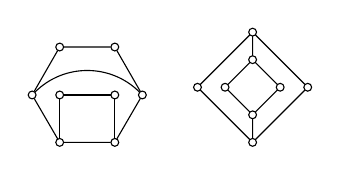
\begin{tikzpicture}[scale=0.7]
\node (p1) at (0,0) [scale=0.3,shape=circle,draw=black,fill=white] {};
\node (p2) at (1,0) [scale=0.3,shape=circle,draw=black,fill=white] {};
\node (p3) at (1.5,0.86) [scale=0.3,shape=circle,draw=black,fill=white] {};
\node (p4) at (1,1.73) [scale=0.3,shape=circle,draw=black,fill=white] {};
\node (p5) at (0,1.73) [scale=0.3,shape=circle,draw=black,fill=white] {};
\node (p6) at (-0.5,0.86) [scale=0.3,shape=circle,draw=black,fill=white] {};
\node (p7) at (0,0.86) [scale=0.3,shape=circle,draw=black,fill=white] {};
\node (p8) at (1,0.86) [scale=0.3,shape=circle,draw=black,fill=white] {};
\draw (p1) -- (p2) -- (p3) -- (p4) -- (p5) -- (p6) -- (p1);
\draw (p1) -- (p7) -- (p8) -- (p2);
\draw (p6) to [bend left=45] (p3);
\node (p9) at (3.5,0) [scale=0.3,shape=circle,draw=black,fill=white] {};
\node (p10) at (4.5,1) [scale=0.3,shape=circle,draw=black,fill=white] {};
\node (p11) at (3.5,2) [scale=0.3,shape=circle,draw=black,fill=white] {};
\node (p12) at (2.5,1) [scale=0.3,shape=circle,draw=black,fill=white] {};
\node (p13) at (3.5,0.5) [scale=0.3,shape=circle,draw=black,fill=white] {};
\node (p14) at (4,1) [scale=0.3,shape=circle,draw=black,fill=white] {};
\node (p15) at (3.5,1.5) [scale=0.3,shape=circle,draw=black,fill=white] {};
\node (p16) at (3,1) [scale=0.3,shape=circle,draw=black,fill=white] {};
\draw (p9) -- (p10) -- (p11) -- (p12) -- (p9);
\draw (p13) -- (p14) -- (p15) -- (p16) -- (p13);
\draw (p9) -- (p13);
\draw (p11) -- (p15);
\end{tikzpicture}\]

%id 37
%topic GRAPHS_PRUFER
Установите соответствие (не обязательно биекцию) между деревьями на рисунке и кодами Прюфера.
\[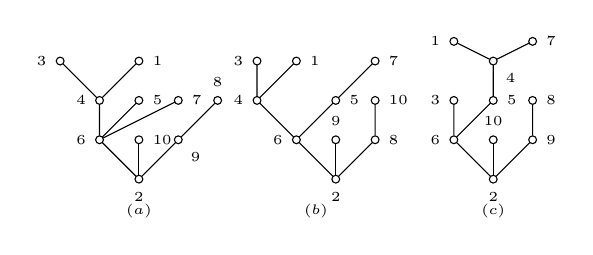
\begin{tikzpicture}[scale=0.5]
\node (p1) at (0,3) [scale=0.3,shape=circle,draw=black,fill=white,label=0:\tiny{$1$}] {};
\node (p2) at (0,0) [scale=0.3,shape=circle,draw=black,fill=white,label=-90:\tiny{$2$}] {};
\node (p3) at (-2,3) [scale=0.3,shape=circle,draw=black,fill=white,label=180:\tiny{$3$}] {};
\node (p4) at (-1,2) [scale=0.3,shape=circle,draw=black,fill=white,label=180:\tiny{$4$}] {};
\node (p5) at (0,2) [scale=0.3,shape=circle,draw=black,fill=white,label=0:\tiny{$5$}] {};
\node (p6) at (-1,1) [scale=0.3,shape=circle,draw=black,fill=white,label=180:\tiny{$6$}] {};
\node (p7) at (1,2) [scale=0.3,shape=circle,draw=black,fill=white,label=0:\tiny{$7$}] {};
\node (p8) at (2,2) [scale=0.3,shape=circle,draw=black,fill=white,label=90:\tiny{$8$}] {};
\node (p9) at (1,1) [scale=0.3,shape=circle,draw=black,fill=white,label=-45:\tiny{$9$}] {};
\node (p10) at (0,1) [scale=0.3,shape=circle,draw=black,fill=white,label=0:\tiny{$10$}] {};
\draw (p2) -- (p6) -- (p4) -- (p3);
\draw (p4) -- (p1);
\draw (p6) -- (p5);
\draw (p6) -- (p7);
\draw (p2) -- (p10);
\draw (p2) -- (p9) -- (p8);
\draw (0,-0.8) node {\emph{\tiny{$(a)$}}};
\node (p11) at (4,3) [scale=0.3,shape=circle,draw=black,fill=white,label=0:\tiny{$1$}] {};
\node (p12) at (5,0) [scale=0.3,shape=circle,draw=black,fill=white,label=-90:\tiny{$2$}] {};
\node (p13) at (3,3) [scale=0.3,shape=circle,draw=black,fill=white,label=180:\tiny{$3$}] {};
\node (p14) at (3,2) [scale=0.3,shape=circle,draw=black,fill=white,label=180:\tiny{$4$}] {};
\node (p15) at (5,2) [scale=0.3,shape=circle,draw=black,fill=white,label=0:\tiny{$5$}] {};
\node (p16) at (4,1) [scale=0.3,shape=circle,draw=black,fill=white,label=180:\tiny{$6$}] {};
\node (p17) at (6,3) [scale=0.3,shape=circle,draw=black,fill=white,label=0:\tiny{$7$}] {};
\node (p18) at (6,1) [scale=0.3,shape=circle,draw=black,fill=white,label=0:\tiny{$8$}] {};
\node (p19) at (5,1) [scale=0.3,shape=circle,draw=black,fill=white,label=90:\tiny{$9$}] {};
\node (p20) at (6,2) [scale=0.3,shape=circle,draw=black,fill=white,label=0:\tiny{$10$}] {};
\draw (p12) -- (p16) -- (p14) -- (p13);
\draw (p14) -- (p11);
\draw (p16) -- (p15) -- (p17);
\draw (p12) -- (p19);
\draw (p12) -- (p18) -- (p20);
\draw (4.5,-0.8) node {\emph{\tiny{$(b)$}}};
\node (p21) at (8,3.5) [scale=0.3,shape=circle,draw=black,fill=white,label=180:\tiny{$1$}] {};
\node (p22) at (9,0) [scale=0.3,shape=circle,draw=black,fill=white,label=-90:\tiny{$2$}] {};
\node (p23) at (8,2) [scale=0.3,shape=circle,draw=black,fill=white,label=180:\tiny{$3$}] {};
\node (p24) at (9,3) [scale=0.3,shape=circle,draw=black,fill=white,label=-45:\tiny{$4$}] {};
\node (p25) at (9,2) [scale=0.3,shape=circle,draw=black,fill=white,label=0:\tiny{$5$}] {};
\node (p26) at (8,1) [scale=0.3,shape=circle,draw=black,fill=white,label=180:\tiny{$6$}] {};
\node (p27) at (10,3.5) [scale=0.3,shape=circle,draw=black,fill=white,label=0:\tiny{$7$}] {};
\node (p28) at (10,2) [scale=0.3,shape=circle,draw=black,fill=white,label=0:\tiny{$8$}] {};
\node (p29) at (10,1) [scale=0.3,shape=circle,draw=black,fill=white,label=0:\tiny{$9$}] {};
\node (p30) at (9,1) [scale=0.3,shape=circle,draw=black,fill=white,label=90:\tiny{$10$}] {};
\draw (p22) -- (p26) -- (p23);
\draw (p22) -- (p30);
\draw (p26) -- (p25) -- (p24) -- (p21);
\draw (p24) -- (p27);
\draw (p22) -- (p29) -- (p28);
\draw (9,-0.8) node {\emph{\tiny{$(c)$}}};
\end{tikzpicture}\]
\begin{enumerate}
\item[(a)] (4,6,4,5,6,2,9,2);
\item[(b)] (4,4,6,6,6,2,9,2);
\item[(c)] (4,4,6,5,6,2,2,10).
\end{enumerate}% Ответ: дереву (a) соответствует код (b), дереву (c) соответствует код (a), дереву (b) и коду (c) ничего не соответствует.


%id 38
%topic GRAPHS_COUNTING_ISOMORPHIC
Пусть $V = \{1,2,3,4,5,6,7,8\}$. Сколько существует графов, изоморфных графу $G$ на рисунке, на множестве вершин $V$ (сам граф $G$ также считается)?% ответ: 8!/4
\[\begin{tikzpicture}[scale=0.7]
\node (p1) at (-1,0) [scale=0.3,shape=circle,draw=black,fill=white,label=90:\tiny{$1$}] {};
\node (p2) at (0,0) [scale=0.3,shape=circle,draw=black,fill=white,label=90:\tiny{$2$}] {};
\node (p3) at (1,0) [scale=0.3,shape=circle,draw=black,fill=white,label=90:\tiny{$3$}] {};
\node (p4) at (2,0) [scale=0.3,shape=circle,draw=black,fill=white,label=90:\tiny{$4$}] {};
\node (p5) at (3,0) [scale=0.3,shape=circle,draw=black,fill=white,label=90:\tiny{$5$}] {};
\node (p6) at (4,0) [scale=0.3,shape=circle,draw=black,fill=white,label=90:\tiny{$6$}] {};
\node (p7) at (5,0) [scale=0.3,shape=circle,draw=black,fill=white,label=90:\tiny{$7$}] {};
\node (p8) at (6,0) [scale=0.3,shape=circle,draw=black,fill=white,label=90:\tiny{$8$}] {};
\draw (p2) -- (p3) -- (p4) -- (p5) -- (p6) -- (p7);
\draw (2.5,-0.5) node {\tiny{Граф $G$.}};
\end{tikzpicture}\]


%id 39
%topic PIGEONHOLE
Предположим, на листике тетради в клетку ученик произвольно в узлах клеточек проставил $5$ точек. Необходимо доказать, что как минимум один отрезок с вершинами в этих точках пройдет через узел клеточки.


%id 40
%topic INDUCTION
Докажите, что предпоследняя цифра десятичной записи любой степени тройки чётна.


%id 41
%topic POTENTIALS
На кольцевой дороге стоят бензоколонки. Общее количество бензина в них достаточно, чтобы объехать круг. Докажите, что автомобиль с пустым баком может стартовать от некоторой бензоколонки и, заправляясь по дороге, объехать весь круг. (Бак достаточно большой.)


%id 42
%topic INDUCTION
Назовём раскраску рёбер дерева \emph{правильной}, если ни в какой вершине дерева не сходятся два ребра одного цвета (т.е. из каждой вершины дерева выходит букет разноцветных рёбер). Докажите методом математической индукции, что если $k\in\bbN$ и у произвольного дерева из каждой вершины выходят не более чем $k$ рёбер, то у дерева существует правильная раскраска, задействующая не более $k$ цветов.


%id 43
%topic INCLEXCL
Используя формулу включений-исключений, найдите формулу для количества различных ($\neq$ неизоморфных!) графов на множестве вершин $\{1,\,2,\,\ldots,\,n\}$, в которых нет изолированных вершин.

%id 44
%topic GRAPHS_TREES_AND_FORESTS
Существует ли унициклический граф, последовательность степеней вершин которого будет равна  $(1,1,1,1,1,1,2,3,3,4,4)?$ Если да, то постройте такой граф.

%id 45
%topic GRAPHS_TREES_AND_FORESTS
%similar to 44
Существует ли унициклический граф, последовательность степеней вершин которого будет равна
$(1,1,1,1,1,1,1,2,4,4,5)?$ Если да, то постройте такой граф.

%id 46
%topic GRAPHS_TREES_AND_FORESTS
%similar to 44
Существует ли унициклический граф, последовательность степеней вершин которого будет равна
$(1,1,1,1,1,1,2,3,3,3,5)?$ Если да, то постройте такой граф.

%id 47
%topic GRAPHS_TREES_AND_FORESTS
Сколько существует попарно неизоморфных помеченных унициклических графов на $n\ge 9$ вершинах с циклом длины $7$?

%id 48
%topic GRAPHS_COUNTING_ISOMORPHIC
Сколько различных \emph{помеченных} деревьев соответствуют непомеченному дереву на рисунке?
\begin{center}
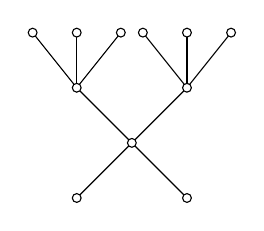
\begin{tikzpicture}[scale=0.7]
\draw (0,0) -- (1,1) -- (0,2) -- (-0.8,3);
\draw (2,0) -- (1,1) -- (2,2) -- (2.8,3);
\draw (2,3) -- (2,2);
\draw (1.2,3) -- (2,2);
\draw (0.8,3) -- (0,2);
\draw (0,3) -- (0,2);
\filldraw [fill=white] (0,0) circle (0.08);
\filldraw [fill=white] (2,0) circle (0.08);
\filldraw [fill=white] (1,1) circle (0.08);
\filldraw [fill=white] (2,2) circle (0.08);
\filldraw [fill=white] (0,2) circle (0.08);
\filldraw [fill=white] (0.8,3) circle (0.08);
\filldraw [fill=white] (0,3) circle (0.08);
\filldraw [fill=white] (-0.8,3) circle (0.08);
\filldraw [fill=white] (1.2,3) circle (0.08);
\filldraw [fill=white] (2,3) circle (0.08);
\filldraw [fill=white] (2.8,3) circle (0.08);
\end{tikzpicture}
\end{center}

%id 49
%topic GRAPHS_COUNTING_ISOMORPHIC
%similar to 48
Сколько различных \emph{помеченных} деревьев соответствуют непомеченному дереву на рисунке?
\begin{center}
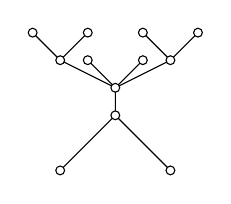
\begin{tikzpicture}[scale=0.7]
\draw (0,0) -- (1,1) -- (1,1.5) -- (0,2) -- (-0.5,2.5);
\draw (2,0) -- (1,1);
\draw (1,1.5) -- (2,2) -- (2.5,2.5);
\draw (0.5,2.5) -- (0,2);
\draw (0.5,2) -- (1,1.5);
\draw (1.5,2) -- (1,1.5);
\draw (1.5,2.5) -- (2,2);
\filldraw [fill=white] (0,0) circle (0.08);
\filldraw [fill=white] (2,0) circle (0.08);
\filldraw [fill=white] (1,1) circle (0.08);
\filldraw [fill=white] (1,1.5) circle (0.08);
\filldraw [fill=white] (0,2) circle (0.08);
\filldraw [fill=white] (0.5,2) circle (0.08);
\filldraw [fill=white] (1.5,2) circle (0.08);
\filldraw [fill=white] (2,2) circle (0.08);
\filldraw [fill=white] (-0.5,2.5) circle (0.08);
\filldraw [fill=white] (0.5,2.5) circle (0.08);
\filldraw [fill=white] (1.5,2.5) circle (0.08);
\filldraw [fill=white] (2.5,2.5) circle (0.08);
\end{tikzpicture}
\end{center}

%id 50
%topic GRAPHS_TREES_AND_FORESTS
Докажите, что количество помеченных лесов на $n$~вершинах с $r$~компонентами, каждая из которых содержит ровно по одной вершине из множества $ \{1, \ldots, r\} $, в точности $rn^{n-1-r}$~штук.

%id 51
%topic GRAPHS_TREES_AND_FORESTS
Докажите, что количество классов изоморфизма деревьев с $n$ вершинами (т.~е. количество различных деревьев с $n$
незанумерованными вершинами) меньше $4^n$.

%id 52
%topic GRAPHS_TREES_AND_FORESTS
Пусть $T_n$ обозначает число помеченных деревьев с $n$~вершинами. Докажите тождество \[2(n-1)T_n=\Sum_{k=1}^{n-1}C_n^k k(n-k) T_kT_{n-k}.\]

%id 53
%topic GRAPHS_COUNTING_ISOMORPHIC
Сколько существует графов, изоморфных графу $G$ на рисунке, на множестве вершин $\{1,2,\ldots,8\}$ (сам граф $G$ также считается)?% ответ: 8!/4
\[\begin{tikzpicture}[scale=0.7]
\node (p1) at (0,0) [scale=0.3,shape=circle,draw=black,fill=white,label=-90:\tiny{$1$}] {};
\node (p2) at (1,0) [scale=0.3,shape=circle,draw=black,fill=white,label=-90:\tiny{$2$}] {};
\node (p3) at (1.5,0.86) [scale=0.3,shape=circle,draw=black,fill=white,label=-45:\tiny{$3$}] {};
\node (p4) at (1,1.72) [scale=0.3,shape=circle,draw=black,fill=white,label=90:\tiny{$4$}] {};
\node (p5) at (0,1.72) [scale=0.3,shape=circle,draw=black,fill=white,label=90:\tiny{$5$}] {};
\node (p6) at (-0.5,0.86) [scale=0.3,shape=circle,draw=black,fill=white,label=180:\tiny{$6$}] {};
\node (p7) at (2.5,0.86) [scale=0.3,shape=circle,draw=black,fill=white,label=-90:\tiny{$7$}] {};
\node (p8) at (3.5,0.86) [scale=0.3,shape=circle,draw=black,fill=white,label=-90:\tiny{$8$}] {};
\draw (p2) -- (p5);
\draw (p1) -- (p4);
\draw (p1) -- (p2) -- (p3) -- (p4) -- (p5) -- (p6) -- (p1);
\draw (p3) -- (p7) -- (p8);
\draw (1.5,-0.6) node {\tiny{Граф $G$.}};
\end{tikzpicture}\]%Ответ: (3/5)8!.


%id 54
%topic GRAPHS_ADVANCED
При каких натуральных $n$ у графа на $n$ вершинах может быть ровно $(n-1)$ центральная вершина?


%id 55
%topic GRAPHS_ADVANCED
\emph{Диаметральной цепью} в графе называется кратчайшая цепь, соединяющая произвольную пару вершин, находящихся на расстоянии диаметра графа. Докажите, что в дереве любые две диаметральные цепи имеют хотя бы одну общую вершину. Верно ли это утверждение для произвольных связных графов?

%id 56
%topic GRAPHS_GREEDY_ALGORITHM
Вершины графа ниже занумерованы по возрастанию слева направо, сверху вниз (номера вершин обозначены на рисунке). Запишите, как этот граф будет раскрашен жадным алгоритмом. Использует ли при этом алгоритм наименьшее возможное для данного графа число цветов? Если да, то докажите, что в меньшее число цветов граф раскрасить нельзя.
\[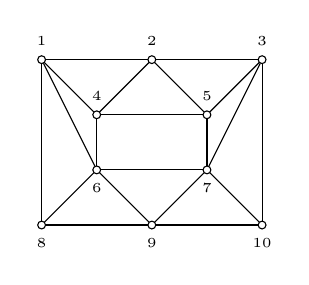
\begin{tikzpicture}[scale=0.7]
 \node (vrtx 1) at (0,0) [scale=0.3,shape=circle,draw=black,fill=white,label=90:\tiny{$1$}] {};
 \node (vrtx 2) at (2,0) [scale=0.3,shape=circle,draw=black,fill=white,label=90:\tiny{$2$}] {};
 \node (vrtx 3) at (4,0) [scale=0.3,shape=circle,draw=black,fill=white,label=90:\tiny{$3$}] {};
 \node (vrtx 4) at (1,-1) [scale=0.3,shape=circle,draw=black,fill=white,label=90:\tiny{$4$}] {};
 \node (vrtx 5) at (3,-1) [scale=0.3,shape=circle,draw=black,fill=white,label=90:\tiny{$5$}] {};
 \node (vrtx 6) at (1,-2) [scale=0.3,shape=circle,draw=black,fill=white,label=-90:\tiny{$6$}] {};
 \node (vrtx 7) at (3,-2) [scale=0.3,shape=circle,draw=black,fill=white,label=-90:\tiny{$7$}] {};
 \node (vrtx 8) at (0,-3) [scale=0.3,shape=circle,draw=black,fill=white,label=-90:\tiny{$8$}] {};
 \node (vrtx 9) at (2,-3) [scale=0.3,shape=circle,draw=black,fill=white,label=-90:\tiny{$9$}] {};
 \node (vrtx 10) at (4,-3) [scale=0.3,shape=circle,draw=black,fill=white,label=-90:\tiny{$10$}] {};
 \draw (vrtx 1) -- (vrtx 2);
 \draw (vrtx 2) -- (vrtx 3);
 \draw (vrtx 1) -- (vrtx 8);
 \draw (vrtx 1) -- (vrtx 4);
 \draw (vrtx 2) -- (vrtx 4);
 \draw (vrtx 2) -- (vrtx 5);
 \draw (vrtx 3) -- (vrtx 5);
 \draw (vrtx 3) -- (vrtx 10);
 \draw (vrtx 4) -- (vrtx 6);
 \draw (vrtx 5) -- (vrtx 7);
 \draw (vrtx 6) -- (vrtx 7);
 \draw (vrtx 6) -- (vrtx 8);
 \draw (vrtx 8) -- (vrtx 9);
 \draw (vrtx 9) -- (vrtx 10);
 \draw (vrtx 6) -- (vrtx 9);
 \draw (vrtx 7) -- (vrtx 9);
 \draw (vrtx 4) -- (vrtx 5);
 \draw (vrtx 7) -- (vrtx 10);
 \draw (vrtx 1) --  (vrtx 6);
 \draw (vrtx 3) --  (vrtx 7);
 \end{tikzpicture}\]


%id 57
%topic GRAPHS_GREEDY_ALGORITHM
%similar to 56
Вершины графа ниже занумерованы по возрастанию слева направо, сверху вниз (номера вершин обозначены на рисунке). Запишите, как этот граф будет раскрашен жадным алгоритмом. Использует ли при этом алгоритм наименьшее возможное для данного графа число цветов? Если да, то докажите, что в меньшее число цветов граф раскрасить нельзя.
\[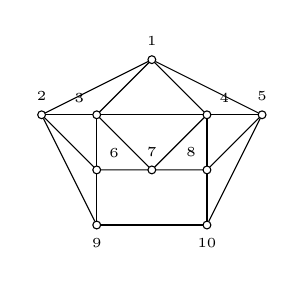
\begin{tikzpicture}[scale=0.7]
 \node (vrtx 1) at (2,0) [scale=0.3,shape=circle,draw=black,fill=white,label=90:\tiny{$1$}] {};
 \node (vrtx 2) at (0,-1) [scale=0.3,shape=circle,draw=black,fill=white,label=90:\tiny{$2$}] {};
 \node (vrtx 3) at (1,-1) [scale=0.3,shape=circle,draw=black,fill=white,label=135:\tiny{$3$}] {};
 \node (vrtx 4) at (3,-1) [scale=0.3,shape=circle,draw=black,fill=white,label=45:\tiny{$4$}] {};
 \node (vrtx 5) at (4,-1) [scale=0.3,shape=circle,draw=black,fill=white,label=90:\tiny{$5$}] {};
 \node (vrtx 6) at (1,-2) [scale=0.3,shape=circle,draw=black,fill=white,label=45:\tiny{$6$}] {};
 \node (vrtx 7) at (2,-2) [scale=0.3,shape=circle,draw=black,fill=white,label=90:\tiny{$7$}] {};
 \node (vrtx 8) at (3,-2) [scale=0.3,shape=circle,draw=black,fill=white,label=110:\tiny{$8$}] {};
 \node (vrtx 9) at (1,-3) [scale=0.3,shape=circle,draw=black,fill=white,label=-90:\tiny{$9$}] {};
 \node (vrtx 10) at (3,-3) [scale=0.3,shape=circle,draw=black,fill=white,label=-90:\tiny{$10$}] {};
 \draw (vrtx 1) -- (vrtx 3);
 \draw (vrtx 1) -- (vrtx 4);
 \draw (vrtx 3) -- (vrtx 4);
 \draw (vrtx 2) -- (vrtx 3);
 \draw (vrtx 4) -- (vrtx 5);
 \draw (vrtx 3) -- (vrtx 7);
 \draw (vrtx 7) -- (vrtx 4);
 \draw (vrtx 7) -- (vrtx 6);
 \draw (vrtx 2) -- (vrtx 6);
 \draw (vrtx 7) -- (vrtx 8);
 \draw (vrtx 8) -- (vrtx 5);
 \draw (vrtx 2) -- (vrtx 9);
 \draw (vrtx 10) -- (vrtx 9);
 \draw (vrtx 10) -- (vrtx 5);
 \draw (vrtx 6) -- (vrtx 9);
 \draw (vrtx 8) -- (vrtx 10);
 \draw (vrtx 3) -- (vrtx 6);
 \draw (vrtx 4) -- (vrtx 8);
 \draw (vrtx 1) -- (vrtx 2);
 \draw (vrtx 1) -- (vrtx 5);
 \end{tikzpicture}\]

%id 58
%topic GRAPHS_COLORINGS_ADVANCED
Назовём граф $G=(V,E)$ на $n$ вершинах \emph{$k$-критическим}, если $\chi(G)=k$, и при этом при удалении любой вершины хроматическое число графа уменьшается. Докажите, что $|E|\ge n(k-1)/2$.

%id 59
%topic GRAPHS_COLORINGS_ADVANCED
Найдите хроматическое число и хроматический индекс графа на рисунке. Ответ обоснуйте.
\[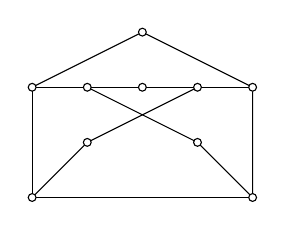
\begin{tikzpicture}[scale=0.7][scale=0.8]
 \node (vrtx 1) at (2,0) [scale=0.3,shape=circle,draw=black,fill=white] {};
 \node (vrtx 2) at (0,-1) [scale=0.3,shape=circle,draw=black,fill=white] {};
 \node (vrtx 3) at (1,-1) [scale=0.3,shape=circle,draw=black,fill=white] {};
 \node (vrtx 4) at (2,-1) [scale=0.3,shape=circle,draw=black,fill=white] {};
 \node (vrtx 5) at (3,-1) [scale=0.3,shape=circle,draw=black,fill=white] {};
 \node (vrtx 6) at (4,-1) [scale=0.3,shape=circle,draw=black,fill=white] {};
 \node (vrtx 7) at (1,-2) [scale=0.3,shape=circle,draw=black,fill=white] {};
 \node (vrtx 8) at (3,-2) [scale=0.3,shape=circle,draw=black,fill=white] {};
 \node (vrtx 9) at (0,-3) [scale=0.3,shape=circle,draw=black,fill=white] {};
 \node (vrtx 10) at (4,-3) [scale=0.3,shape=circle,draw=black,fill=white] {};
 \draw (vrtx 1) -- (vrtx 2);
 \draw (vrtx 1) -- (vrtx 6);
 \draw (vrtx 2) -- (vrtx 3);
 \draw (vrtx 3) -- (vrtx 4);
 \draw (vrtx 4) -- (vrtx 5);
 \draw (vrtx 5) -- (vrtx 6);
 \draw (vrtx 2) -- (vrtx 9);
 \draw (vrtx 9) -- (vrtx 10);
 \draw (vrtx 6) -- (vrtx 10);
 \draw (vrtx 9) -- (vrtx 7);
 \draw (vrtx 7) -- (vrtx 5);
 \draw (vrtx 3) -- (vrtx 8);
 \draw (vrtx 8) -- (vrtx 10);
 \end{tikzpicture}\]

%id 60
%topic GRAPHS_COLORINGS_ADVANCED
Найдите хроматическое число и хроматический индекс графа на рисунке. Ответ обоснуйте.
\[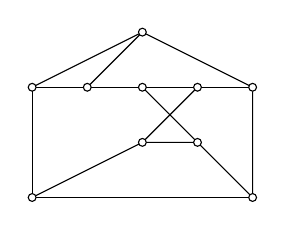
\begin{tikzpicture}[scale=0.7][scale=0.8]
 \node (vrtx 1) at (2,0) [scale=0.3,shape=circle,draw=black,fill=white] {};
 \node (vrtx 2) at (0,-1) [scale=0.3,shape=circle,draw=black,fill=white] {};
 \node (vrtx 3) at (1,-1) [scale=0.3,shape=circle,draw=black,fill=white] {};
 \node (vrtx 4) at (2,-1) [scale=0.3,shape=circle,draw=black,fill=white] {};
 \node (vrtx 5) at (3,-1) [scale=0.3,shape=circle,draw=black,fill=white] {};
 \node (vrtx 6) at (4,-1) [scale=0.3,shape=circle,draw=black,fill=white] {};
 \node (vrtx 7) at (2,-2) [scale=0.3,shape=circle,draw=black,fill=white] {};
 \node (vrtx 8) at (3,-2) [scale=0.3,shape=circle,draw=black,fill=white] {};
 \node (vrtx 9) at (0,-3) [scale=0.3,shape=circle,draw=black,fill=white] {};
 \node (vrtx 10) at (4,-3) [scale=0.3,shape=circle,draw=black,fill=white] {};
 \draw (vrtx 1) -- (vrtx 2);
 \draw (vrtx 1) -- (vrtx 6);
 \draw (vrtx 2) -- (vrtx 3);
 \draw (vrtx 3) -- (vrtx 4);
 \draw (vrtx 4) -- (vrtx 5);
 \draw (vrtx 5) -- (vrtx 6);
 \draw (vrtx 2) -- (vrtx 9);
 \draw (vrtx 9) -- (vrtx 10);
 \draw (vrtx 6) -- (vrtx 10);
 \draw (vrtx 9) -- (vrtx 7);
 \draw (vrtx 7) -- (vrtx 5);
 \draw (vrtx 4) -- (vrtx 8);
 \draw (vrtx 8) -- (vrtx 10);
 \draw (vrtx 1) -- (vrtx 3);
 \draw (vrtx 7) -- (vrtx 8);
 \end{tikzpicture}\]

%id 61
%topic GRAPHS_GREEDY_ALGORITHM
%similar to 56
Вершины графа ниже занумерованы по возрастанию слева направо (номера вершин обозначены на рисунке), сверху вниз. Запишите, как этот граф будет раскрашен жадным алгоритмом. Использует ли при этом алгоритм наименьшее возможное для данного графа число цветов? Если да, то докажите, что в меньшее число цветов граф раскрасить нельзя. Если нет, то приведите новую нумерацию вершин графа, при которой алгоритм построит оптимальную раскраску.
\[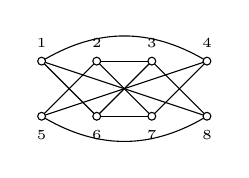
\begin{tikzpicture}[scale=0.7]
 \node (vrtx 1) at (0,0) [scale=0.3,shape=circle,draw=black,fill=white,label=90:\tiny{$1$}] {};
 \node (vrtx 2) at (1,0) [scale=0.3,shape=circle,draw=black,fill=white,label=90:\tiny{$2$}] {};
 \node (vrtx 3) at (2,0) [scale=0.3,shape=circle,draw=black,fill=white,label=90:\tiny{$3$}] {};
 \node (vrtx 4) at (3,0) [scale=0.3,shape=circle,draw=black,fill=white,label=90:\tiny{$4$}] {};
 \node (vrtx 5) at (0,-1) [scale=0.3,shape=circle,draw=black,fill=white,label=-90:\tiny{$5$}] {};
 \node (vrtx 6) at (1,-1) [scale=0.3,shape=circle,draw=black,fill=white,label=-90:\tiny{$6$}] {};
 \node (vrtx 7) at (2,-1) [scale=0.3,shape=circle,draw=black,fill=white,label=-90:\tiny{$7$}] {};
 \node (vrtx 8) at (3,-1) [scale=0.3,shape=circle,draw=black,fill=white,label=-90:\tiny{$8$}] {};
  \draw (vrtx 2) -- (vrtx 3);
 \draw (vrtx 1) -- (vrtx 6);
 \draw (vrtx 1) -- (vrtx 8);
 \draw (vrtx 6) -- (vrtx 7);
 \draw (vrtx 5) -- (vrtx 2);
 \draw (vrtx 5) -- (vrtx 4);
 \draw (vrtx 2) -- (vrtx 7);
 \draw (vrtx 6) -- (vrtx 3);
 \draw (vrtx 3) -- (vrtx 8);
 \draw (vrtx 4) -- (vrtx 7);
 \draw (vrtx 1) to [bend left=30] (vrtx 4);
 \draw (vrtx 5) to [bend left=-30] (vrtx 8);
\end{tikzpicture}\]


%id 62
%topic GRAPHS_GREEDY_ALGORITHM
%similar to 56
Вершины графа ниже занумерованы по возрастанию слева направо (номера вершин обозначены на рисунке), сверху вниз. Запишите, как этот граф будет раскрашен жадным алгоритмом. Использует ли при этом алгоритм наименьшее возможное для данного графа число цветов? Если да, то докажите, что в меньшее число цветов граф раскрасить нельзя. Если нет, то приведите новую нумерацию вершин графа, при которой алгоритм построит оптимальную раскраску.
\[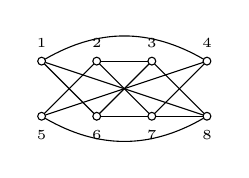
\begin{tikzpicture}[scale=0.7]
 \node (vrtx 1) at (0,0) [scale=0.3,shape=circle,draw=black,fill=white,label=90:\tiny{$1$}] {};
 \node (vrtx 2) at (1,0) [scale=0.3,shape=circle,draw=black,fill=white,label=90:\tiny{$2$}] {};
 \node (vrtx 3) at (2,0) [scale=0.3,shape=circle,draw=black,fill=white,label=90:\tiny{$3$}] {};
 \node (vrtx 4) at (3,0) [scale=0.3,shape=circle,draw=black,fill=white,label=90:\tiny{$4$}] {};
 \node (vrtx 5) at (0,-1) [scale=0.3,shape=circle,draw=black,fill=white,label=-90:\tiny{$5$}] {};
 \node (vrtx 6) at (1,-1) [scale=0.3,shape=circle,draw=black,fill=white,label=-90:\tiny{$6$}] {};
 \node (vrtx 7) at (2,-1) [scale=0.3,shape=circle,draw=black,fill=white,label=-90:\tiny{$7$}] {};
 \node (vrtx 8) at (3,-1) [scale=0.3,shape=circle,draw=black,fill=white,label=-90:\tiny{$8$}] {};
  \draw (vrtx 2) -- (vrtx 3);
 \draw (vrtx 1) -- (vrtx 6);
 \draw (vrtx 1) -- (vrtx 8);
 \draw (vrtx 6) -- (vrtx 7);
 \draw (vrtx 5) -- (vrtx 2);
 \draw (vrtx 5) -- (vrtx 4);
 \draw (vrtx 2) -- (vrtx 7);
 \draw (vrtx 6) -- (vrtx 3);
 \draw (vrtx 3) -- (vrtx 8);
 \draw (vrtx 4) -- (vrtx 7);
 \draw (vrtx 7) -- (vrtx 8);
 \draw (vrtx 1) to [bend left=30] (vrtx 4);
 \draw (vrtx 5) to [bend left=-30] (vrtx 8);
 \end{tikzpicture}\]


%id 63
%topic GRAPHS_COLORINGS_ADVANCED
Дан связный граф c $6$ вершинами. В каких пределах может меняться его хроматическое число? В каких пределах может меняться хроматический индекс этого графа? Для каждого предельного значения хроматического числа/индекса необходимо привести пример, на котором это значение достигается.

%id 64
%topic GRAPHS_COLORINGS_ADVANCED
%similar to 63
Дан связный граф c $7$ вершинами. В каких пределах может меняться его хроматическое число? В каких пределах может меняться хроматический индекс этого графа? Для каждого предельного значения хроматического числа/индекса необходимо привести пример, на котором это значение достигается.

%id 65
%topic GRAPHS_COLORINGS_ADVANCED
%similar to 63
Дан связный граф c $8$ вершинами. В каких пределах может меняться его хроматическое число? В каких пределах может меняться хроматический индекс этого графа? Для каждого предельного значения хроматического числа/индекса необходимо привести пример, на котором это значение достигается.

%id 66
%topic GRAPHS_PLANARITY
Планарен ли следующий граф? Если да, то нарисуйте его без самопересечений, если нет, то найдите в нём подграф, гомеоморфный $K_{3,3}.$
\[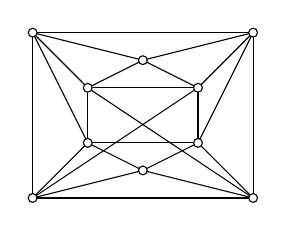
\begin{tikzpicture}[scale=0.7]
\draw (0,0) -- (0,3);
\draw (0,0) -- (4,0);
\draw (4,0) -- (4,3);
\draw (0,3) -- (4,3);
\draw (0,3) -- (2,2.5);
\draw (4,3) -- (2,2.5);
\draw (2,2.5) -- (1,2);
\draw (2,2.5) -- (3,2);
\draw (1,2) -- (1,1);
\draw (1,2) -- (3,2);
\draw (3,2) -- (3,1);
\draw (1,1) -- (3,1);
\draw (1,1) -- (2,0.5);
\draw (3,1) -- (2,0.5);
\draw (0,0) -- (2,0.5);
\draw (2,0.5) -- (4,0);
\draw (0,3) -- (1,2);
\draw (0,3) -- (1,1);
\draw (4,3) -- (3,2);
\draw (4,3) -- (3,1);
\draw (4,0) -- (3,1);
\draw (4,0) -- (1,2);
\draw (0,0) -- (3,2);
\draw (0,0) -- (1,1);
\filldraw [fill=white]  (0,0) circle (0.08);
\filldraw [fill=white] (4,0) circle (0.08);
\filldraw [fill=white] (2,0.5) circle (0.08);
\filldraw [fill=white] (1,1) circle (0.08);
\filldraw [fill=white] (3,1) circle (0.08);
\filldraw [fill=white] (1,2) circle (0.08);
\filldraw [fill=white] (3,2) circle (0.08);
\filldraw [fill=white] (2,2.5) circle (0.08);
\filldraw [fill=white] (0,3) circle (0.08);
\filldraw [fill=white] (4,3) circle (0.08);
\end{tikzpicture}\]

%id 67
%topic GRAPHS_PLANARITY
%similar to 66
Планарен ли следующий граф? Если да, то нарисуйте его без самопересечений, если нет, то найдите в нём подграф, гомеоморфный $K_{3,3}.$
\[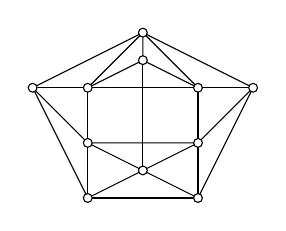
\begin{tikzpicture}[scale=0.7]
\draw (1,0) -- (0,2);
\draw (0,2) -- (2,3);
\draw (2,3) -- (4,2);
\draw (4,2) -- (3,0);
\draw (1,0) -- (3,0);
\draw (1,0) -- (1,1);
\draw (1,1) -- (1,2);
\draw (1,2) -- (2,3);
\draw (3,0) -- (3,1);
\draw (3,1) -- (3,2);
\draw (3,2) -- (2,3);
\draw (0,2) -- (1,2) -- (3,2) -- (4,2);
\draw (2,3) -- (2,2.5) -- (1,2);
\draw (2,2.5) -- (3,2);
\draw (1,0) -- (2,0.5) -- (1,1) -- (3,1) -- (2,0.5) -- (3,0);
\draw (0,2) -- (1,1);
\draw (4,2) -- (3,1);
\draw (2,0.5) -- (2,2.5);
\filldraw [fill=white] (1,0) circle (0.08);
\filldraw [fill=white] (3,0) circle (0.08);
\filldraw [fill=white] (2,0.5) circle (0.08);
\filldraw [fill=white] (1,1) circle (0.08);
\filldraw [fill=white] (3,1) circle (0.08);
\filldraw [fill=white] (0,2) circle (0.08);
\filldraw [fill=white] (1,2) circle (0.08);
\filldraw [fill=white] (3,2) circle (0.08);
\filldraw [fill=white] (4,2) circle (0.08);
\filldraw [fill=white] (2,2.5) circle (0.08);
\filldraw [fill=white] (2,3) circle (0.08);
\end{tikzpicture}\]

%id 68
%topic GRAPHS_PLANARITY
%similar to 66
Планарен ли следующий граф? Если да, то нарисуйте его без самопересечений, если нет, то найдите в нём подграф, гомеоморфный $K_{3,3}.$
\[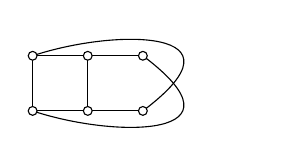
\begin{tikzpicture}[scale=0.7]
\draw (0,0) -- (0,1);
\draw (0,0) -- (1,0);
\draw (0,1) -- (1,1);
\draw (1,0) -- (1,1);
\draw (1,1) -- (2,1);
\draw (1,0) -- (2,0);
\draw (0,1) .. controls (1.5,1.5) and (4,1.5) .. (2,0);
\draw (0,0) .. controls (1.5,-0.5) and (4,-0.5) .. (2,1);
\filldraw [fill=white] (0,0) circle (0.08);
\filldraw [fill=white] (1,0) circle (0.08);
\filldraw [fill=white] (0,1) circle (0.08);
\filldraw [fill=white] (1,1) circle (0.08);
\filldraw [fill=white] (2,0) circle (0.08);
\filldraw [fill=white] (2,1) circle (0.08);
\end{tikzpicture}\]

%id 69
%topic GRAPHS_PLANARITY
%similar to 66
Планарен ли следующий граф? Если да, то нарисуйте его без самопересечений, если нет, то найдите в нём подграф, гомеоморфный $K_{3,3}.$
\[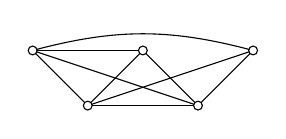
\begin{tikzpicture}[scale=0.7]
\draw (0,1) -- (1,0);
\draw (0,1) -- (3,0);
\draw (0,1) -- (2,1);
\draw (1,0) -- (2,1);
\draw (1,0) -- (4,1);
\draw (1,0) -- (3,0);
\draw (2,1) -- (3,0);
\draw (3,0) -- (4,1);
\draw (0,1) to [bend left=15] (4,1);
\filldraw [fill=white] (0,1) circle (0.08);
\filldraw [fill=white] (1,0) circle (0.08);
\filldraw [fill=white] (2,1) circle (0.08);
\filldraw [fill=white] (3,0) circle (0.08);
\filldraw [fill=white] (4,1) circle (0.08);
\end{tikzpicture}\]

%id 70
%topic GRAPHS_PLANARITY
%similar to 66
Планарен ли следующий граф? Если да, то нарисуйте его без самопересечений, если нет, то найдите в нём подграф, гомеоморфный $K_{3,3}.$
\[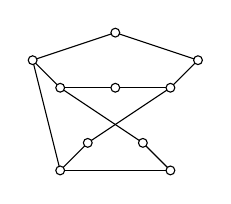
\begin{tikzpicture}[scale=0.7]
\draw (0.5,0) -- (2.5,0);
\draw (3,2) -- (1.5,2.5) -- (0,2) -- (0.5,0);
\draw (0.5,0) -- (1,0.5) -- (2.5,1.5) -- (3,2);
\draw (2.5,0) -- (2,0.5) -- (0.5,1.5) -- (0,2);
\draw (0.5,1.5) -- (1.5,1.5) -- (2.5,1.5);
\filldraw [fill=white] (0,2) circle (0.08);
\filldraw [fill=white] (0.5,0) circle (0.08);
\filldraw [fill=white] (2.5,0) circle (0.08);
\filldraw [fill=white] (1,0.5) circle (0.08);
\filldraw [fill=white] (2,0.5) circle (0.08);
\filldraw [fill=white] (0.5,1.5) circle (0.08);
\filldraw [fill=white] (1.5,1.5) circle (0.08);
\filldraw [fill=white] (2.5,1.5) circle (0.08);
\filldraw [fill=white] (3,2) circle (0.08);
\filldraw [fill=white] (1.5,2.5) circle (0.08);
\end{tikzpicture}\]


%id 71
%topic GRAPHS_PLANARITY
%similar to 66
Планарен ли следующий граф? Если да, то нарисуйте его без самопересечений, если нет, то найдите в нём подграф, гомеоморфный $K_{3,3}.$
\[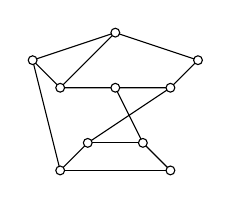
\begin{tikzpicture}[scale=0.7]
\draw (0.5,0) -- (2.5,0);
\draw (3,2) -- (1.5,2.5) -- (0,2) -- (0.5,0);
\draw (0.5,0) -- (1,0.5) -- (2.5,1.5) -- (3,2);
\draw (0,2) -- (0.5,1.5) -- (1.5,1.5) -- (2.5,1.5);
\draw (0.5,1.5) -- (1.5,2.5);
\draw (1,0.5) -- (2,0.5);
\draw (2.5,0) -- (2,0.5) -- (1.5,1.5);
\filldraw [fill=white] (0,2) circle (0.08);
\filldraw [fill=white] (0.5,0) circle (0.08);
\filldraw [fill=white] (2.5,0) circle (0.08);
\filldraw [fill=white] (1,0.5) circle (0.08);
\filldraw [fill=white] (2,0.5) circle (0.08);
\filldraw [fill=white] (0.5,1.5) circle (0.08);
\filldraw [fill=white] (1.5,1.5) circle (0.08);
\filldraw [fill=white] (2.5,1.5) circle (0.08);
\filldraw [fill=white] (3,2) circle (0.08);
\filldraw [fill=white] (1.5,2.5) circle (0.08);
\end{tikzpicture}\]

%id 72
%topic GRAPHS_PLANARITY
Из двух представленных ниже графов ровно один планарен. Перерисуйте планарный граф без пересечений рёбер, а в непланарном графе найдите подграф, гомеоморфный $K_{3,3}.$
\[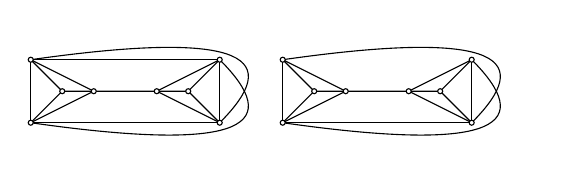
\begin{tikzpicture}[scale=0.4]
\draw (0,0) -- (0,2) -- (6,2) -- (6,0) --(0,0);
\draw (0,2) -- (1,1) -- (2,1) -- (4,1) -- (5,1) -- (6,2);
\draw (0,0) -- (1,1);
\draw (0,0) -- (2,1);
\draw (6,0) -- (4,1);
\draw (6,0) -- (5,1);
\draw (0,2) -- (2,1);
\draw (6,2) -- (4,1);
\draw (0,2) .. controls (7,3) and (8,2) .. (6,0);
\draw (6,2) .. controls (8,0) and (7,-1) .. (0,0);
\draw (8,0) -- (8,2);
\draw (14,2) -- (14,0) --(8,0);
\draw (8,2) -- (9,1) -- (10,1) -- (12,1) -- (13,1) -- (14,2);
\draw (8,0) -- (9,1);
\draw (8,0) -- (10,1);
\draw (14,0) -- (12,1);
\draw (14,0) -- (13,1);
\draw (8,2) -- (10,1);
\draw (14,2) -- (12,1);
\draw (8,2) .. controls (15,3) and (16,2) .. (14,0);
\draw (14,2) .. controls (16,0) and (15,-1) .. (8,0);
\filldraw [fill=white] (0,0) circle (0.08);
\filldraw [fill=white] (0,2) circle (0.08);
\filldraw [fill=white] (1,1) circle (0.08);
\filldraw [fill=white] (2,1) circle (0.08);
\filldraw [fill=white] (4,1) circle (0.08);
\filldraw [fill=white] (5,1) circle (0.08);
\filldraw [fill=white] (6,0) circle (0.08);
\filldraw [fill=white] (6,2) circle (0.08);
\filldraw [fill=white] (8,0) circle (0.08);
\filldraw [fill=white] (8,2) circle (0.08);
\filldraw [fill=white] (9,1) circle (0.08);
\filldraw [fill=white] (10,1) circle (0.08);
\filldraw [fill=white] (12,1) circle (0.08);
\filldraw [fill=white] (13,1) circle (0.08);
\filldraw [fill=white] (14,0) circle (0.08);
\filldraw [fill=white] (14,2) circle (0.08);
\end{tikzpicture}\]


%id 73
%topic PIGEONHOLE
Квадратная таблица $(2n+1)\times(2n+1)$, где $n\in\mathbb{N}$, заполнена числами от $1$ до $2n+1$ так, что в каждой строке и в каждом столбце представлены все эти числа. Докажите, что если это расположение симметрично относительно диагонали таблицы, то на этой диагонали тоже представлены все эти числа.

%id 74
%topic INDUCTION
Докажите, что число, состоящее из $3^n$ единиц, где $n\in\mathbb{N}$, делится на $3^n$.

%id 75
%topic NUMBER_THEORY_EULER_FERMAT_THEOREM
Числа $p$ и $q$ --- нечётные простые, $2^p - 1 \equiv 0 \pmod q$. Докажите, что $q - 1 \equiv 0 \pmod p$.

%id 76
%topic NUMBER_THEORY_EULER_FERMAT_THEOREM
Докажите, что если $x^2+1$ делится на нечётное простое $p$, то $p=4k+1$.


%id 77
%topic POTENTIALS
Есть $n$ прямых общего положения и $n$ точек, где $n\in\mathbb{N}$. Докажите, что их можно занумеровать так, что перпендикуляры, опущенные из этих точек на прямые с теми же номерами, не будут пересекаться.


%id 78
%topic NUMBER_THEORY_EULER_FERMAT_THEOREM
Пусть $p$ --- простое нечётное число, не равное $5$. Применив малую теорему Ферма, докажите, что среди чисел, записываемых только единицами, есть число, которое делится на $p$.

%id 79
%topic ENUMERATION
Весёлая компания из $10$ супружеских пар разбивается на $5$ групп по $4$ человека для лодочной прогулки так, чтобы в одной лодке оказались двое мужчин и двое женщин. Во скольких случаях Леонид Иванович Комбинаторщиков (один из участников Весёлой компании) окажется в одной лодке со своей женой?


%id 80
%topic GRAPHS_CLIQUES
Объединением графов $G'=(V',\,E')$ и $G''=(V'',\, E'')$ называется граф $G=(V,\,E)$, такой, что $V=V'\cup V''$ и $E=E'\cup E''$. Пусть $\omega'$ и $\omega''$ — кликовое число графов $G'$ и $G''$ соответственно. Дайте достижимую нижнюю оценку на кликовое число графа $G$. Докажите, что для любых натуральных $k',\,k''$ бывают графы $G'$ и $G''$, для которых $\omega(G')=k'$, $\omega(G'')=k''$, и $\omega(G)\ge k'\cdot k''$.


%id 81
%topic GRAPHS_PIGEONHOLE
Пусть $k,n\in\bbN$ и $3\le k\le n$. Докажите, что если в графе на $n$ вершинах степень каждой вершины не меньше чем $(n-k+2)$, то граф обязательно содержит цикл, длина которого не превосходит $k$.


%id 82
%topic GRAPHS_PRUFER
Установите соответствие (не обязательно биекцию) между деревьями на рисунке и кодами Прюфера.
\[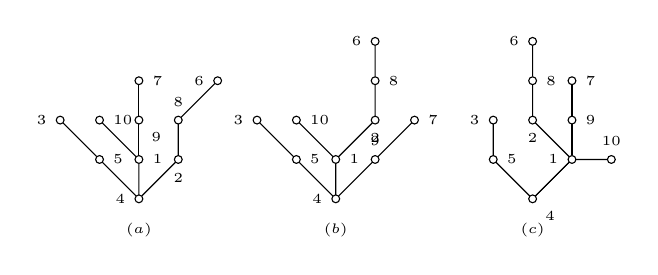
\begin{tikzpicture}[scale=0.5]
\node (p1) at (0,1) [scale=0.3,shape=circle,draw=black,fill=white,label=0:\tiny{$1$}] {};
\node (p2) at (1,1) [scale=0.3,shape=circle,draw=black,fill=white,label=-90:\tiny{$2$}] {};
\node (p3) at (-2,2) [scale=0.3,shape=circle,draw=black,fill=white,label=180:\tiny{$3$}] {};
\node (p4) at (0,0) [scale=0.3,shape=circle,draw=black,fill=white,label=180:\tiny{$4$}] {};
\node (p5) at (-1,1) [scale=0.3,shape=circle,draw=black,fill=white,label=0:\tiny{$5$}] {};
\node (p6) at (2,3) [scale=0.3,shape=circle,draw=black,fill=white,label=180:\tiny{$6$}] {};
\node (p7) at (0,3) [scale=0.3,shape=circle,draw=black,fill=white,label=0:\tiny{$7$}] {};
\node (p8) at (1,2) [scale=0.3,shape=circle,draw=black,fill=white,label=90:\tiny{$8$}] {};
\node (p9) at (0,2) [scale=0.3,shape=circle,draw=black,fill=white,label=-45:\tiny{$9$}] {};
\node (p10) at (-1,2) [scale=0.3,shape=circle,draw=black,fill=white,label=0:\tiny{$10$}] {};
\draw (p3) -- (p5) -- (p4) -- (p2) -- (p8) -- (p6);
\draw (p4) -- (p1) -- (p10);
\draw (p1) -- (p9) -- (p7);
\draw (0,-0.8) node {\emph{\tiny{$(a)$}}};
\node (p11) at (5,1) [scale=0.3,shape=circle,draw=black,fill=white,label=0:\tiny{$1$}] {};
\node (p12) at (6,2) [scale=0.3,shape=circle,draw=black,fill=white,label=-90:\tiny{$2$}] {};
\node (p13) at (3,2) [scale=0.3,shape=circle,draw=black,fill=white,label=180:\tiny{$3$}] {};
\node (p14) at (5,0) [scale=0.3,shape=circle,draw=black,fill=white,label=180:\tiny{$4$}] {};
\node (p15) at (4,1) [scale=0.3,shape=circle,draw=black,fill=white,label=0:\tiny{$5$}] {};
\node (p16) at (6,4) [scale=0.3,shape=circle,draw=black,fill=white,label=180:\tiny{$6$}] {};
\node (p17) at (7,2) [scale=0.3,shape=circle,draw=black,fill=white,label=0:\tiny{$7$}] {};
\node (p18) at (6,3) [scale=0.3,shape=circle,draw=black,fill=white,label=0:\tiny{$8$}] {};
\node (p19) at (6,1) [scale=0.3,shape=circle,draw=black,fill=white,label=90:\tiny{$9$}] {};
\node (p20) at (4,2) [scale=0.3,shape=circle,draw=black,fill=white,label=0:\tiny{$10$}] {};
\draw (p13) -- (p15) -- (p14) -- (p19) -- (p17);
\draw (p14) -- (p11) -- (p20);
\draw (p11) -- (p12) -- (p18) -- (p16);
\draw (5,-0.8) node {\emph{\tiny{$(b)$}}};
\node (p21) at (11,1) [scale=0.3,shape=circle,draw=black,fill=white,label=180:\tiny{$1$}] {};
\node (p22) at (10,2) [scale=0.3,shape=circle,draw=black,fill=white,label=-90:\tiny{$2$}] {};
\node (p23) at (9,2) [scale=0.3,shape=circle,draw=black,fill=white,label=180:\tiny{$3$}] {};
\node (p24) at (10,0) [scale=0.3,shape=circle,draw=black,fill=white,label=-45:\tiny{$4$}] {};
\node (p25) at (9,1) [scale=0.3,shape=circle,draw=black,fill=white,label=0:\tiny{$5$}] {};
\node (p26) at (10,4) [scale=0.3,shape=circle,draw=black,fill=white,label=180:\tiny{$6$}] {};
\node (p27) at (11,3) [scale=0.3,shape=circle,draw=black,fill=white,label=0:\tiny{$7$}] {};
\node (p28) at (10,3) [scale=0.3,shape=circle,draw=black,fill=white,label=0:\tiny{$8$}] {};
\node (p29) at (11,2) [scale=0.3,shape=circle,draw=black,fill=white,label=0:\tiny{$9$}] {};
\node (p30) at (12,1) [scale=0.3,shape=circle,draw=black,fill=white,label=90:\tiny{$10$}] {};
\draw (p23) -- (p25) -- (p24) -- (p21) -- (p30);
\draw (p24) -- (p21) -- (p22) -- (p28) -- (p26);
\draw (p21) -- (p29) -- (p27);
\draw (10,-0.8) node {\emph{\tiny{$(c)$}}};
\end{tikzpicture}\]
\begin{enumerate}
\item[(a)] (5,4,8,9,2,1,4,1);
\item[(b)] (5,4,8,9,2,1,1,4);
\item[(c)] (5,4,8,9,2,4,1,1).
\end{enumerate}% Ответ: дереву (a) соответствует код (c), дереву (b) соответствует код (a), дереву (c) и коду (b) ничего не соответствует.

%id 83
%topic GRAPHS_EULERIAN
Рёберным графом графа $G$ называется граф $G'$, такой, что вершины графа $G'$ соответствуют рёбрам $G$, и две вершины в $G'$ смежны тогда и только тогда, когда соответствующие им рёбра в $G$ имеют общий конец. Докажите или опровергните утверждение: «если в $G$ есть эйлеров цикл, то и в $G'$ также есть эйлеров цикл».

%id 84
%topic GRAPHS_DEBRUIJN
Постройте \textbf{троичную} последовательность де Брёйна порядка два, начинающуюся с «$220\ldots$». Сделайте это, найдя эйлеров цикл в соответствующем графе.

%id 85
%topic ENUMERATION
В группе $20$ студентов, из которых $5$ математиков-олимпиадников, $10$ обычных студентов и $5$… кхм… не слишком сильных. Сколькими способами студентов можно разбить на две команды для матбоя, так, чтобы в каждой команде оказался хотя бы один олимпиадник и все не слишком хорошие студенты не попали в одну команду?

%id 86
%topic INCLEXCL
Окружность разбита на $2015$ равных пронумерованных дуг. Сколькими способами можно раскрасить эти дуги в красный и синий цвета, так, чтобы ни одна красная дуга не была окружена двумя синими дугами? Раскраски, отличающиеся друг от друга поворотами окружности, считайте разными.

%id 87
%topic GRAPHS_DEBRUIJN
С помощью графа де\,Брёйна постройте двоичную последовательность де\,Брёйна порядка $4$, заканчивающуюся последовательностью 101111.

%id 88
%topic GRAPHS_DEBRUIJN
%similar to 87
С помощью графа де\,Брёйна постройте двоичную последовательность де\,Брёйна порядка $4$, заканчивающуюся последовательностью 000110.

%id 89
%topic GRAPHS_EULERIAN
Эйлеров ли этот граф? Если да, то найдите в нём эйлеров цикл, если нет, то найдите минимальное число рёбер, которые необходимо из него удалить, чтобы он стал эйлеровым. Ответ обоснуйте.
\[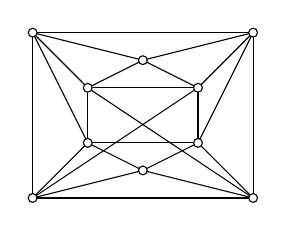
\begin{tikzpicture}[scale=0.7]
\draw (0,0) -- (0,3);
\draw (0,0) -- (4,0);
\draw (4,0) -- (4,3);
\draw (0,3) -- (4,3);
\draw (0,3) -- (2,2.5);
\draw (4,3) -- (2,2.5);
\draw (2,2.5) -- (1,2);
\draw (2,2.5) -- (3,2);
\draw (1,2) -- (1,1);
\draw (1,2) -- (3,2);
\draw (3,2) -- (3,1);
\draw (1,1) -- (3,1);
\draw (1,1) -- (2,0.5);
\draw (3,1) -- (2,0.5);
\draw (0,0) -- (2,0.5);
\draw (2,0.5) -- (4,0);
\draw (0,3) -- (1,2);
\draw (0,3) -- (1,1);
\draw (4,3) -- (3,2);
\draw (4,3) -- (3,1);
\draw (4,0) -- (3,1);
\draw (4,0) -- (1,2);
\draw (0,0) -- (3,2);
\draw (0,0) -- (1,1);
\filldraw [fill=white]  (0,0) circle (0.08);
\filldraw [fill=white] (4,0) circle (0.08);
\filldraw [fill=white] (2,0.5) circle (0.08);
\filldraw [fill=white] (1,1) circle (0.08);
\filldraw [fill=white] (3,1) circle (0.08);
\filldraw [fill=white] (1,2) circle (0.08);
\filldraw [fill=white] (3,2) circle (0.08);
\filldraw [fill=white] (2,2.5) circle (0.08);
\filldraw [fill=white] (0,3) circle (0.08);
\filldraw [fill=white] (4,3) circle (0.08);
\end{tikzpicture}\]


%id 90
%topic GRAPHS_EULERIAN
%similar to 89
Эйлеров ли этот граф? Если да, то найдите в нём эйлеров цикл, если нет, то найдите минимальное число рёбер, которые необходимо из него удалить, чтобы он стал эйлеровым. Ответ обоснуйте.
\[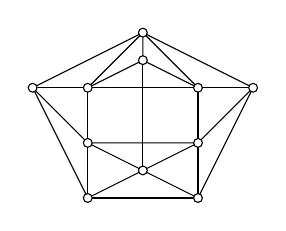
\begin{tikzpicture}[scale=0.7]
\draw (1,0) -- (0,2);
\draw (0,2) -- (2,3);
\draw (2,3) -- (4,2);
\draw (4,2) -- (3,0);
\draw (1,0) -- (3,0);
\draw (1,0) -- (1,1);
\draw (1,1) -- (1,2);
\draw (1,2) -- (2,3);
\draw (3,0) -- (3,1);
\draw (3,1) -- (3,2);
\draw (3,2) -- (2,3);
\draw (0,2) -- (1,2) -- (3,2) -- (4,2);
\draw (2,3) -- (2,2.5) -- (1,2);
\draw (2,2.5) -- (3,2);
\draw (1,0) -- (2,0.5) -- (1,1) -- (3,1) -- (2,0.5) -- (3,0);
\draw (0,2) -- (1,1);
\draw (4,2) -- (3,1);
\draw (2,0.5) -- (2,2.5);
\filldraw [fill=white] (1,0) circle (0.08);
\filldraw [fill=white] (3,0) circle (0.08);
\filldraw [fill=white] (2,0.5) circle (0.08);
\filldraw [fill=white] (1,1) circle (0.08);
\filldraw [fill=white] (3,1) circle (0.08);
\filldraw [fill=white] (0,2) circle (0.08);
\filldraw [fill=white] (1,2) circle (0.08);
\filldraw [fill=white] (3,2) circle (0.08);
\filldraw [fill=white] (4,2) circle (0.08);
\filldraw [fill=white] (2,2.5) circle (0.08);
\filldraw [fill=white] (2,3) circle (0.08);
\end{tikzpicture}\]


%id 91
%topic GRAPHS_COLORINGS_ADVANCED
Докажите, что если граф невозможно правильно раскрасить в $k-1$ цвет, то для любой его правильной раскраски в $k$ цветов существует путь, в котором встречается ровно по одной вершине каждого цвета.

%id 92
%topic GRAPHS_COLORINGS_ADVANCED
Докажите, что если максимальный несамопересекающийся путь в графе проходит через $d$ вершин,
то граф можно правильно раскрасить в $d$ цветов.

%id 93
%topic GRAPHS_COLORINGS_ADVANCED
Докажите, что если максимальный нечётный несамопересекающийся цикл в графе проходит через $d-1$ вершину, то граф можно правильно раскрасить в $d$ цветов.

%id 94
%topic GRAPHS_TREES_AND_FORESTS
Пусть $T_1,\ldots,T_r$ --- деревья, множества вершин которых не~пересекаются. Сколько есть деревьев, множество вершин которых есть объединение множества вершин этих $r$ деревьев, и которые содержат $T_1,\ldots, T_r?$

%id 95
%topic GRAPHS_EULERIAN
Все рёбра связного графа раскрашены в два цвета. Из каждой вершины выходит поровну рёбер обоих цветов. Докажите, что тогда из любой вершины до любой другой можно добраться, каждый раз меняя цвет ребра.

%id 96
%topic NUMBER_THEORY_EULER_FERMAT_THEOREM
Рассмотрим вычеты по модулю $27$. Какие значения может принимать порядок элементов по этому модулю? Для каких элементов по модулю $27$ определено понятие порядка?

%id 97
%topic NUMBER_THEORY_LINEAR_EQUATIONS
Решите сравнение $42x\equiv 15\pmod{61}$.

%id 98
%topic NUMBER_THEORY_LINEAR_EQUATIONS
%similar to 97
Решите сравнение $37x\equiv 15\pmod{59}$.

%id 99
%topic NUMBER_THEORY_LINEAR_EQUATIONS_ADVANCED
Решите сравнение $76x\equiv 40\pmod{100}$. Решение необходимо записать по модулю $100$.

%id 100
%topic NUMBER_THEORY_LINEAR_EQUATIONS_ADVANCED
%similar to 99
Решите сравнение $90x\equiv 114\pmod{213}.$ Решение необходимо записать по модулю $213$.

%id 101
%topic NUMBER_THEORY_LINEAR_EQUATIONS_ADVANCED
%similar to 99
Решите сравнение $36x\equiv 24\pmod{120}.$ Решение необходимо записать по модулю $120$.

%id 102
%topic NUMBER_THEORY_LINEAR_EQUATIONS
%similar to 97
Решите сравнение $78x\equiv 189\pmod{213}$. Решение необходимо записать по модулю $213$.

%id 103
%topic NUMBER_THEORY_EULER_FERMAT_THEOREM
Существует ли $k$, такое, что $3^k$ оканчивается на $\ldots000081$?

%id 104
%topic NUMBER_THEORY_EULER_FERMAT_THEOREM
%similar to 103
Существует ли $k$, такое, что ${13}^k$ оканчивается на $\ldots0000169$?

%id 105
%topic NUMBER_THEORY_EULER_FERMAT_THEOREM
%similar to 103
Существует ли $k$, такое, что $7^k$ оканчивается на $\ldots000049$?

%id 106
%topic NUMBER_THEORY_EULER_FERMAT_THEOREM
%similar to 103
Существует ли $k$, такое, что ${11}^k$ оканчивается на $\ldots0000121$?

%id 107
%topic INCLEXCL
Модифицируя формулу включений-исключений, докажите следующую формулу:
\[n! \cdot x_1 x_2\ldots x_n = (x_1 + x_2+ \ldots + x_n)^n -\]
\[- \sum_{1 \leqslant i_1<i_2<\ldots < i_{n-1} \leqslant n} (x_{i_1} + x_{i_2}+ \ldots + x_{i_{n-1}})^n +\]
\[+ \sum_{1\leqslant i_1<i_2<\ldots < i_{n-2} \leqslant n} (x_{i_1} + x_{i_2}+ \ldots + x_{i_{n-2}})^n - \ldots + (-1)^{n-1} \sum_{i=1}^n x_i^n.\]
Указание: посчитайте двумя способами число упорядоченных мономов степени $n$ от переменных $x_1,x_2,\ldots,x_n$, в которых встречаются все переменные.

%id 108
%topic INCLEXCL
Найдите количество всех сюръективных отображений из $n$ элементного множества в $k$ элементное множество при $k\leqslant n$.


%id 109
%topic ENUMERATION
Сколькими способами можно посадить за круглый стол с $9$ местами $3$ англичан, $3$ французов и $3$ турок так, чтобы никакие \emph{три} соотечественника не сидели рядом? Рассадки, совмещающиеся поворотами круглого стола считаются одинаковыми. Все люди в задаче различны. Тот же вопрос, но в случае, когда никакие два соотечественника не сидят рядом?

%id 110
%topic ENUMERATION
%similar to 79
Весёлая компания из $20$ супружеских пар разбивается на $5$ групп по $4$ человека для лодочной прогулки так, чтобы в одной лодке оказались двое мужчин и двое женщин. Во скольких случаях Леонид Иванович Комбинаторщиков и Степан Витальевич Дискретщиков (оба из Весёлой компании) окажутся каждый в одной лодке со своей женой?

%id 111
%topic GRAPHS_HAMILTONIAN
Для множества $X$ вершин графа будем через $\calN(X)$ обозначать множество всех вершин, смежных с  вершинами из $X$ (кроме вершин самого множества $X$).
Пусть граф $G$ содержит такое \emph{независимое} множество вершин $X\subseteq V(G)$, что $|X|>|\calN(X)|$. Докажите, что в $G$ нет гамильтоновых циклов.

%id 112
%topic GRAPHS_HAMILTONIAN
%similar to 111
Для множества $X$ вершин графа будем через $\calK(X)$ будем обозначать количество компонент связности, на которые распадается граф при удалении всех вершин множества $X$ (вершины удаляются вместе со всеми рёбрами, которые шли в них).
Докажите, что, если граф $G$ гамильтонов, то для любого непустого подмножества вершин $A\subseteq V(G)$ выполнено неравенство $\calK(A)\le |A|.$

%id 113
%topic GRAPHS_HAMILTONIAN
Гамильтонов ли следующий граф? (Если да, то найдите в нём гамильтонов цикл; если нет — докажите.)
\[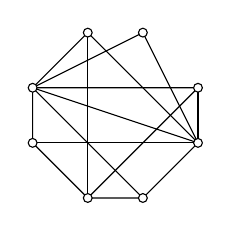
\begin{tikzpicture}[scale=0.7]
\draw (0,0) -- (-1,1) -- (-1,2) -- (0,3) -- (2,1) -- (1,0) -- (0,0);
\draw (-1,2) -- (2,2) -- (0,0);
\draw (1,0) -- (-1,2) -- (2,1) -- (1,3) -- (-1,2);
\draw (0,0) -- (0,3);
\draw (2,1) -- (2,2);
\draw (-1,1) -- (2,1);
\filldraw [fill=white] (0,0) circle (0.08);
\filldraw [fill=white] (1,0) circle (0.08);
\filldraw [fill=white] (-1,1) circle (0.08);
\filldraw [fill=white] (2,1) circle (0.08);
\filldraw [fill=white] (-1,2) circle (0.08);
\filldraw [fill=white] (2,2) circle (0.08);
\filldraw [fill=white] (0,3) circle (0.08);
\filldraw [fill=white] (1,3) circle (0.08);
\end{tikzpicture}\]

%id 114
%topic GRAPHS_HAMILTONIAN
%similar to 113
Гамильтонов ли следующий граф? (Если да, то найдите в нём гамильтонов цикл; если нет — докажите.)
\[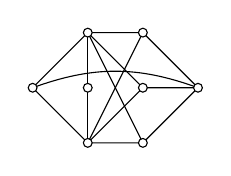
\begin{tikzpicture}[scale=0.7]
\draw (0,0) -- (-1,1) -- (0,2) -- (1,2) -- (2,1) -- (1,0) -- (0,0);
\draw (0,0) -- (0,1) -- (0,2);
\draw (0,0) -- (1,2);
\draw (2,1) -- (1,1) -- (0,0);
\draw (1,0) -- (0,2);
\draw (1,1) -- (0,2);
\draw (-1,1) to [bend left=20] (2,1);
\filldraw [fill=white] (0,0) circle (0.08);
\filldraw [fill=white] (0,1) circle (0.08);
\filldraw [fill=white] (-1,1) circle (0.08);
\filldraw [fill=white] (1,1) circle (0.08);
\filldraw [fill=white] (2,1) circle (0.08);
\filldraw [fill=white] (0,2) circle (0.08);
\filldraw [fill=white] (1,2) circle (0.08);
\filldraw [fill=white] (1,0) circle (0.08);
\end{tikzpicture}\]

%id 115
%topic GRAPHS_HAMILTONIAN
%similar to 114
Гамильтонов ли следующий граф? (Если да, то найдите в нём гамильтонов цикл; если нет — докажите.)
\[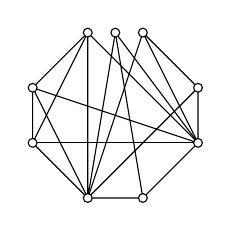
\begin{tikzpicture}[scale=0.7]
\draw (0,3) -- (-1,2) -- (-1,1) -- (0,0) -- (1,0) -- (2,1) -- (2,2) -- (1,3) -- (2,1) -- (0,3) -- (0,0) -- (0.5,3) -- (1,0);
\draw (2,1) -- (-1,2);
\draw (2,1) -- (-1,1);
\draw (0,0) -- (1,3);
\draw (0,0) -- (2,2);
\draw (-1,1) -- (0,3);
\draw (0.5,3) -- (2,1);
\draw (0,0) -- (-1,2);
\filldraw [fill=white] (0,0) circle (0.08);
\filldraw [fill=white] (1,0) circle (0.08);
\filldraw [fill=white] (-1,1) circle (0.08);
\filldraw [fill=white] (-1,2) circle (0.08);
\filldraw [fill=white] (0,3) circle (0.08);
\filldraw [fill=white] (0.5,3) circle (0.08);
\filldraw [fill=white] (1,3) circle (0.08);
\filldraw [fill=white] (2,2) circle (0.08);
\filldraw [fill=white] (2,1) circle (0.08);
\end{tikzpicture}\]

%id 116
%topic GRAPHS_HAMILTONIAN
%similar to 115
Гамильтонов ли следующий граф? (Если да, то найдите в нём гамильтонов цикл; если нет — докажите.)
\[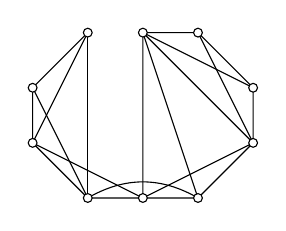
\begin{tikzpicture}[scale=0.7]
\draw (0,3) -- (-1,2) -- (-1,1) -- (0,0) -- (1,0) -- (2,0) -- (3,1) -- (3,2) -- (2,3) -- (1,3) -- (3,1) -- (1,0) -- (1,3);
\draw (1,3) -- (3,2);
\draw (1,3) -- (2,0);
\draw (3,1) -- (2,3);
\draw (1,0) -- (-1,1);
\draw (0,0) -- (-1,2);
\draw (0,0) -- (0,3);
\draw (-1,1) -- (0,3);
\draw (0,0) to [bend left=30] (2,0);
\filldraw [fill=white] (0,0) circle (0.08);
\filldraw [fill=white] (1,0) circle (0.08);
\filldraw [fill=white] (2,0) circle (0.08);
\filldraw [fill=white] (-1,1) circle (0.08);
\filldraw [fill=white] (-1,2) circle (0.08);
\filldraw [fill=white] (0,3) circle (0.08);
\filldraw [fill=white] (1,3) circle (0.08);
\filldraw [fill=white] (2,3) circle (0.08);
\filldraw [fill=white] (3,1) circle (0.08);
\filldraw [fill=white] (3,2) circle (0.08);
\end{tikzpicture}\]

%id 117
%topic GRAPHS_HAMILTONIAN
%similar to 112
Докажите, что граф Петерсена не гамильтонов. Если удалить любую вершину из графа Петерсона, то получается гамильтонов граф. Найдите в каждом таком графе гамильтонов цикл.

%id 118
%topic GRAPHS_HAMILTONIAN
%similar to 116
Гамильтонов ли следующий граф? (Если да, то найдите в нём гамильтонов цикл; если нет — докажите.)
\[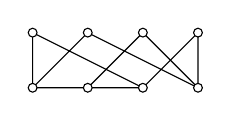
\begin{tikzpicture}[scale=0.7]
\draw (0,0) -- (0,1) -- (2,0) -- (1,0) -- (0,0) -- (1,1) -- (3,0) -- (3,1) -- (2,0);
\draw (1,0) -- (2,1) -- (3,0);
\filldraw [fill=white] (0,0) circle (0.08);
\filldraw [fill=white] (1,0) circle (0.08);
\filldraw [fill=white] (0,1) circle (0.08);
\filldraw [fill=white] (1,1) circle (0.08);
\filldraw [fill=white] (2,0) circle (0.08);
\filldraw [fill=white] (2,1) circle (0.08);
\filldraw [fill=white] (3,0) circle (0.08);
\filldraw [fill=white] (3,1) circle (0.08);
\end{tikzpicture}\]

%id 119
%topic GRAPHS_HAMILTONIAN
%similar to 117
Гамильтонов ли следующий граф? (Если да, то найдите в нём гамильтонов цикл; если нет — докажите.)
\[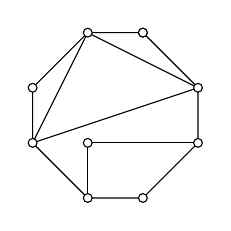
\begin{tikzpicture}[scale=0.7]
\draw (0,0) -- (-1,1) -- (-1,2) -- (0,3) -- (1,3) -- (2,2) -- (2,1) -- (1,0) -- (0,0);
\draw (0,0) -- (0,1);
\draw (0,1) -- (2,1);
\draw (-1,1) -- (2,2) -- (0,3) -- (-1,1);
\filldraw [fill=white] (0,0) circle (0.08);
\filldraw [fill=white] (1,0) circle (0.08);
\filldraw [fill=white] (2,1) circle (0.08);
\filldraw [fill=white] (2,2) circle (0.08);
\filldraw [fill=white] (1,3) circle (0.08);
\filldraw [fill=white] (0,3) circle (0.08);
\filldraw [fill=white] (1,3) circle (0.08);
\filldraw [fill=white] (-1,2) circle (0.08);
\filldraw [fill=white] (-1,1) circle (0.08);
\filldraw [fill=white] (0,1) circle (0.08);
\end{tikzpicture}\]

%id 120
%topic GRAPHS_HAMILTONIAN
%similar to 117
Пусть в связном графе $G$ есть мост (ребро, при удалении которого граф теряет связность). Докажите, что граф $G$ не содержит гамильтонова цикла.

%id 121
%topic NUMBER_THEORY_CHINESE_REMAINDER_THEOREM
%block for 491
%block for 492
%block for 493
Докажите, что $p$ и $p+2$ одновременно просты тогда и только тогда, когда $4((p-1)!+1)+p\equiv 0\pmod{p^2+2p}$.

%id 122
%topic NUMBER_THEORY_EULER_FERMAT_THEOREM
Докажите, что $(p-1)! \equiv -1 \pmod{p}$ тогда и только тогда, когда $p$ --- простое.

%id 123
%topic NUMBER_THEORY_CHINESE_REMAINDER_THEOREM
Найдите все целочисленные решения системы сравнений
\[\left\{
\begin{aligned}
2x&\equiv 4\pmod{6} \\
3x&\equiv 12\pmod{15} \\
\end{aligned}
\right.\]

%id 124
%topic NUMBER_THEORY_CHINESE_REMAINDER_THEOREM
%similar to 123
Укажите все целые числа, удовлетворяющие системе
\[\left\{
\begin{aligned}
x&\equiv 3\pmod{5} \\
x&\equiv 7\pmod{17} \\
\end{aligned}
\right.\]

%id 125
%topic NUMBER_THEORY_CHINESE_REMAINDER_THEOREM
%similar to 123
Укажите все целые числа, удовлетворяющие системе
\[\left\{
\begin{aligned}
x&\equiv 2\pmod{3} \\
x&\equiv 3\pmod{5} \\
x&\equiv 5\pmod{7} \\
\end{aligned}
\right.\]

%id 126
%topic PIGEONHOLE
В классе 25 человек. Известно, что среди любых трех из них есть двое друзей. Докажите, что есть ученик, у которого не менее 12 друзей.

%id 127
%topic INDUCTION
Для любого $x\geq -1$ и натурального $n$ докажите неравенство Бернулли: $(1+x)^n\geq 1+nx$.

%id 128
%topic GREEK
%similar to 1
Заполните все пустые клетки таблицы; в названиях укажите ударение.\\
\begin{tabularx}{\linewidth}{|X|X|X|X|X|X|}\hline
Строчная\newline буква & Прописная\newline буква & Название & Строчная\newline буква & Прописная\newline буква & Название\\\hline
$\psi$ & & &  & $N$ & \\\hline
$\delta$ & & &  & $\Omega$ & \\\hline
$\rho$ & & &  & $H$ & \\\hline
\end{tabularx}


%id 129
%topic CONVERSE
%similar to 5
Сформулируйте утверждение, обратное к теореме Оре (о гамильтоновости графа).

%id 130
%topic GRAPHS_CLIQUES
Постройте граф с максимально возможным количеством рёбер на $8$ вершинах с кликовым числом равным $5$.


%id 131
%topic NUMBER_THEORY_CHINESE_REMAINDER_THEOREM
%similar to 125
Найдите все целочисленные решения системы сравнений
\[\left\{
\begin{aligned}
15x&\equiv 3\pmod{39} \\
21x&\equiv 9\pmod{57} \\
\end{aligned}
\right.\]

%id 132
%topic NUMBER_THEORY_PRIMITIVE_ROOTS
Найдите все первообразные корни по модулю $11$.

%id 133
%topic NUMBER_THEORY_PRIMITIVE_ROOTS
%similar to 132
Найдите все первообразные корни по модулю $17$.

%id 134
%topic NUMBER_THEORY_PRIMITIVE_ROOTS
Существует ли такое $m$, что нет ни одного первообразного корня по модулю $m$? Если да, то приведите пример такого модуля и докажите несуществование первообразного корня по этому модулю; если нет --- докажите.

%id 135
%topic NUMBER_THEORY_PRIMITIVE_ROOTS
Пусть $g$ --- первообразный корень по модулю $m.$ Докажите, что $g^l$ --- первообразный корень тогда и только тогда, когда $(l, \phi(m)) = 1$.

%id 136
%topic NUMBER_THEORY_PRIMITIVE_ROOTS_ADVANCED
Найдите хотя бы один первообразный корень по модулю $27$.

%id 137
%topic NUMBER_THEORY_PRIMITIVE_ROOTS_ADVANCED
%similar to 136
Найдите хотя бы один первообразный корень по модулю $49$.

%id 138
%topic NUMBER_THEORY_PRIMITIVE_ROOTS_ADVANCED
%similar to 136
Найдите хотя бы один первообразный корень по модулю $289$.

%id 139
%topic NUMBER_THEORY_PRIMITIVE_ROOTS_ADVANCED
Найдите хотя бы один первообразный корень по модулю $50$.

%id 140
%topic NUMBER_THEORY_PRIMITIVE_ROOTS_ADVANCED
%similar to 139
Найдите хотя бы один первообразный корень по модулю $98$.

%id 141
%topic NUMBER_THEORY_PRIMITIVE_ROOTS_ADVANCED
%similar to 139
Найдите хотя бы один первообразный корень по модулю $54$.

%id 142
%topic ASYMPTOTICS
Найдите асимптотику величины $\binom{3n+\ln{n}}{2n}$ при $n\to+\infty$. Под нахождением асимптотики понимается нахождение такой функции $f$, между которой и оцениваемой величиной можно было бы поставить знак $\sim$. Ответ принимается только в виде формулы, не содержащей неопределённостей вида $1^{\infty}$, $0^0$, $(\const+0)^\infty$ и пр.

%id 143
%topic ASYMPTOTICS
%similar to 142
Найдите асимптотику величины $\binom{7n}{3n+\ln{n}}$ при $n\to+\infty$. Под нахождением асимптотики понимается нахождение такой функции $f$, между которой и оцениваемой величиной можно было бы поставить знак $\sim$. Ответ принимается только в виде формулы, не содержащей неопределённостей вида $1^{\infty}$, $0^0$, $(\const+0)^\infty$ и пр. %Ответ: \sqrt{7}{24\pi e^{1/3+1/4}} \cdot \left(\frac{7^7}{3^3 4^4}\right)^n (4/3)^{\sqrt{n}} \cdot n^{-1/2}

%id 144
%topic ASYMPTOTICS
%similar to 142
Найдите асимптотику величины $\binom{5n+\ln{n}}{2n}$ при $n\to+\infty$. Под нахождением асимптотики понимается нахождение такой функции $f$, между которой и оцениваемой величиной можно было бы поставить знак $\sim$. Ответ принимается только в виде формулы, не содержащей неопределённостей вида $1^{\infty}$, $0^0$, $(\const+0)^\infty$ и пр.

%id 145
%topic ASYMPTOTICS
%similar to 142
Найдите асимптотику величины $\binom{9n+\ln{n}}{n}$ при $n\to+\infty$. Под нахождением асимптотики понимается нахождение такой функции $f$, между которой и оцениваемой величиной можно было бы поставить знак $\sim$. Ответ принимается только в виде формулы, не содержащей неопределённостей вида $1^{\infty}$, $0^0$, $(\const+0)^\infty$ и пр.

%id 146
%topic ASYMPTOTICS
Пусть $n\to\infty$. Вычислите асимптотику полиномиального коэффициента $P(2n,5n,n,\sqrt{n})=\frac{(8n+\sqrt{n})!}{(2n)!(5n)!n!\sqrt{n}!}$.
Под нахождением асимптотики понимается нахождение такой функции $f$, между которой и оцениваемой величиной можно было бы поставить знак $\sim$. Ответ принимается только в виде формулы, не содержащей неопределённостей вида $1^{\infty}$, $0^0$, $(\const+0)^\infty$ и пр.

%id 147
%topic ASYMPTOTICS
%similar to 146
Пусть  $n\to\infty$. Вычислите асимптотику полиномиального коэффициента $P(7n,2n,n,\sqrt{n})=\frac{(10n+\sqrt{n})!}{(7n)!(2n)!n!\sqrt{n}!}$.
Под нахождением асимптотики понимается нахождение такой функции $f$, между которой и оцениваемой величиной можно было бы поставить знак $\sim$. Ответ принимается только в виде формулы, не содержащей неопределённостей вида $1^{\infty}$, $0^0$, $(\const+0)^\infty$ и пр.

%id 148
%topic ASYMPTOTICS
%similar to 146
Пусть $n\to\infty$. Вычислите асимптотику полиномиального коэффициента $P(n,2n,3n+\sqrt{n},\sqrt{n})=\frac{(6n+2\sqrt{n})!}{n!(2n)!(3n+\sqrt{n})!\sqrt{n}!}$.
Под нахождением асимптотики понимается нахождение такой функции $f$, между которой и оцениваемой величиной можно было бы поставить знак $\sim$. Ответ принимается только в виде формулы, не содержащей неопределённостей вида $1^{\infty}$, $0^0$, $(\const+0)^\infty$ и пр.

%id 149
%topic ASYMPTOTICS
%similar to 146
Пусть $n\to\infty$. Вычислите асимптотику полиномиального коэффициента $P(n+\sqrt{n},5n,3n,\sqrt{n})=\frac{(9n+2\sqrt{n})!}{(n+\sqrt{n})!(5n)!(3n)!\sqrt{n}!}$.
Под нахождением асимптотики понимается нахождение такой функции $f$, между которой и оцениваемой величиной можно было бы поставить знак $\sim$. Ответ принимается только в виде формулы, не содержащей неопределённостей вида $1^{\infty}$, $0^0$, $(\const+0)^\infty$ и пр.

%id 150
%topic ASYMPTOTICS_SIMPLE
Пусть $f,g,h$ — неубывающие функции из $\bbR^{+}$ в $\bbR^{+}$. Пусть $n\to\infty$. Верно ли, что если $f(n)=O(g(n))$ и $g(n)=O(h(n))$, то обязательно $f(n)=O(h(n))$? Если верно, то обоснуйте, опираясь исключительно на определения. Если не верно в общем случае, то приведите соответствующий контрпример.

%id 151
%topic GRAPHS_MATCHINGS
Хирург З.\,А.~Резников планирует удалить графу $K_{n,n}$ несколько рёбер, так, чтобы у графа не осталось ни одного совершенного паросочетания [наличие последних, видимо, портит графу внешность]. Каким минимально возможным количеством рёбер придётся-таки пожертвовать графу? Ответ обоснуйте, опираясь на теорему Холла.

%id 152
%topic GRAPHS_MATCHINGS
Докажите, что в любом двудольном регулярном непустом графе есть хотя бы одно совершенное паросочетание.

%id 153
%topic ASYMPTOTICS_SIMPLE
%similar to 150
Пусть $f,g,h$ — неубывающие функции из $\bbR^{+}$ в $\bbR^{+}$. Пусть $n\to\infty$. Верно ли, что если $f(n)=o(g(n))$ и $g(n)=o(h(n))$, то обязательно $f(n)=o(h(n))$? Если верно, то обоснуйте, опираясь исключительно на определения. Если не верно в общем случае, то приведите соответствующий контрпример.

%id 154
%topic ASYMPTOTICS_SIMPLE
%similar to 150
Пусть $f,g,h$ — неубывающие функции из $\bbR^{+}$ в $\bbR^{+}$. Пусть $n\to\infty$. Верно ли, что если $f(n)=o(g(n))$ и $g(n)=O(h(n))$, то обязательно $f(n)=o(h(n))$? Если верно, то обоснуйте, опираясь исключительно на определения. Если не верно в общем случае, то приведите соответствующий контрпример.

%id 155
%topic ASYMPTOTICS_SIMPLE
%similar to 150
Пусть $f,g,h$ — неубывающие функции из $R^{+}$ в $R^{+}$. Пусть $n\to\infty$. Верно ли, что если $f(n)=O(g(n))$ и $g(n)=o(h(n))$, то обязательно $f(n)=o(h(n))$? Если верно, то обоснуйте, опираясь исключительно на определения. Если не верно в общем случае, то приведите соответствующий контрпример.

%id 156
%topic GREEK
%similar to 1
Заполните все пустые клетки таблицы; в названиях \textbf{укажите ударение}.\\
\begin{tabularx}{\linewidth}{|X|X|X|X|X|X|}\hline
Строчная\newline буква & Прописная\newline буква & Название & Строчная\newline буква & Прописная\newline буква & Название\\\hline
$\tau$ & & &  & $\Xi$ & \\\hline
 & $\Omega$ & &  & $Z$ & \\\hline
$\mu$ & & &  &  & тета \\\hline
\end{tabularx}

%id 157
%topic GRAPHS_MATCHINGS
Пусть в двудольном графе $G$ с долями $X$ и $Y$ существует совершенное паросочетание, и пусть $\deg v\ge t$ для каждой вершины $v\in X$. Докажите, что в $G$ найдутся не менее $t!$ различных совершенных паросочетаний.

%id 158
%topic ASYMPTOTICS_ADVANCED
Функция $n(s)$ задана в виде $n:=\max\{n_0\mid \left(n_0!\right)^{n_0}\le s\}$. Найдите асимптотику этой функции при $s\to\infty$.

%id 159
%topic ASYMPTOTICS_ADVANCED
%similar to 158
Функция $n(s)$ задана в виде $n:=\max\{n_0\mid \left(n_0!\right)^{\ln n_0}\le s\}$. Найдите асимптотику этой функции при $s\to\infty$.

%id 160
%topic ASYMPTOTICS_ADVANCED
%similar to 158
Положим $s(n)=\min\{m\in\mathbb{N}, m\neq 0,1\mid C_n^m\cdot e^{-m^3/(\ln m)^{10}}<1\}$. Найдите асимптотику функции~$s(n)$.

%id 161
%topic ASYMPTOTICS_ADVANCED
%similar to 158
Положим $s(n)=\min\{m\in\mathbb{N}, m\neq 0,1\mid C_n^m\cdot e^{-m^2/(\ln m)^8}<1\}$. Найдите асимптотику для~$s(n)$.


%id 162
%topic NUMBER_THEORY_INDEXES
Решите сравнение $x^{18}\equiv 4\pmod{31}$. Можете без доказательства пользоваться тем, что $3$ — первообразный корень по модулю $31$. Всю таблицу индексов выписывать не обязательно.

%id 163
%topic NUMBER_THEORY_INDEXES
%similar to 162
Решите сравнение $x^{24}\equiv 23\pmod{29}$. Можете без доказательства пользоваться тем, что $2$ — первообразный корень по модулю $29$. Всю таблицу индексов выписывать не обязательно.

%id 164
%topic NUMBER_THEORY_INDEXES
Докажите, что существует элемент порядка ровно $2\cdot 5^{50}$ по модулю $5^{100}$. Приведите пример элемента такого порядка.

%id 165
%topic NUMBER_THEORY_INDEXES
%similar to 164
Докажите, что существует элемент порядка ровно $3\cdot 7^{50}$ по модулю $7^{100}$. Приведите пример элемента такого порядка.

%id 166
%topic NUMBER_THEORY_INDEXES
%similar to 164
Докажите, что существует элемент порядка ровно $5\cdot 11^{100}$ по модулю $11^{200}$. Приведите пример элемента такого порядка.

%id 167
%topic ASYMPTOTICS_ADVANCED
Пусть $p\to\infty$, $s=C_{p^4}^p$ и $n=C_{p^4}^{p^2}$. Найдите функцию~$f(s)$ в записи $n=(e+o(1))^{f(s)}$. Здесь $e=2.71828...$ --- основание натурального логарифма.

%id 168
%topic LINEAR_RECURRENT_RELATIONS
Дан клетчатый прямоугольник размером $n\times 2$, $n\in\bbN$. Обозначим символом $a_n$ число способов замостить этот прямоугольник фигурами двух типов: уголками размером $2\times 2$ и доминошками размера $2\times 1$ (см. рис. 1). Никакие две фигуры не должны перекрываться и каждая клетка прямоугольника должна быть покрыта некоторой фигурой. Выведите линейное рекуррентное соотношение для $a_n$ и укажите начальные условия, необходимые для его корректного задания. Замощения, совмещающиеся отражениями относительно обеих осей симметрии прямоугольника, считаются различными. Считайте, что $a_0=1$. Пример замощения прямоугольника размера $4\times 2$ приведён на рис.2.
\[\begin{tikzpicture}[scale=0.7]
\draw[step=1,black,very thin] (0,0) grid (1,2);
\draw (3,1) -- (4,1) -- (4,2) -- (3,2);
\draw[step=1,black,very thin] (2,0) grid (3,2);
\draw (2,-0.3) node {\footnotesize{Рис. 1. Доминошка и уголок.}};

\filldraw[pattern=north east lines] (8,2) -- (8,0) -- (10,0) -- (10,1) -- (9,1) -- (9,2) -- (8,2);
\filldraw[pattern=horizontal lines] (10,0) -- (12,0) -- (12,2) -- (11,2) -- (11,1) -- (10,1) -- (10,0);
\filldraw[pattern=dots] (9,1) -- (9,2) -- (11,2) -- (11,1) -- (9,1);
\draw[step=1,black,very thin] (8,0) grid (12,2);
\draw (10,-0.3) node {\footnotesize{Рис. 2. Пример замощения прямоугольника $4\times 2.$}};
\end{tikzpicture}\]
%Ответ: $a_{n+3}-2a_{n+2}-a_n=0, a_0=1,a_1=1,a_2=2,a_3=5.$

%id 169
%topic LINEAR_RECURRENT_RELATIONS
%similar to 168
Дан клетчатый прямоугольник размером $n\times 2$, $n\in\bbN$. Обозначим символом $a_n$ число способов замостить этот прямоугольник фигурами двух типов: уголками размером $2\times 2$ и доминошками размера $3\times 1$ (см. рис. 1). Никакие две фигуры не должны перекрываться и каждая клетка прямоугольника должна быть покрыта некоторой фигурой. Выведите линейное рекуррентное соотношение для $a_n$ и укажите начальные условия, необходимые для его корректного задания. Замощения, совмещающиеся отражениями относительно обеих осей симметрии прямоугольника, считаются различными. Считайте, что $a_0=1$. Пример замощения прямоугольника размера $6\times 2$ приведён на рис.2.
\[\begin{tikzpicture}[scale=0.7]
\draw[step=1,black,very thin] (0,0) grid (1,3);
\draw (3,1) -- (4,1) -- (4,2) -- (3,2);
\draw[step=1,black,very thin] (2,0) grid (3,2);
\draw (2,-0.3) node {\footnotesize{Рис. 1. Доминошка и уголок.}};

\filldraw[pattern=north east lines] (7,2) -- (7,0) -- (9,0) -- (9,1) -- (8,1) -- (8,2) -- (7,2);
\filldraw[pattern=horizontal lines] (11,1) -- (12,1) -- (12,0) -- (13,0) -- (13,2) -- (11,2) -- (11,1);
\filldraw[pattern=dots] (9,0) -- (12,0) -- (12,1) -- (9,1) -- (9,0);
\filldraw[pattern=grid] (8,1) -- (11,1) -- (11,2) -- (8,2) -- (8,1);
\draw[step=1,black,very thin] (7,0) grid (13,2);
\draw (10,-0.3) node {\footnotesize{Рис. 2. Пример замощения прямоугольника $6\times 2.$}};
\end{tikzpicture}\]
%Ответ: $a_{n+6}-4a_{n+3}+a_n=0,a_0=1,a_1=a_2=0,a_3=3,a_4=a_5=0,a_6=11$


%id 170
%topic LINEAR_RECURRENT_RELATIONS
Найдите линейное рекуррентное соотношение для последовательности $\{a_n\}_{n=0}^\infty$, где $a_n$ --- количество двоичных слов длины $n$, не содержащих подслова ``110'' и вычислите $a_0$, $a_1$ и $a_2$.

%id 171
%topic LINEAR_RECURRENT_RELATIONS
%similar to 170
Найдите линейное рекуррентное соотношение для последовательности $\{a_n\}_{n=0}^\infty$, где $a_n$ --- количество двоичных слов длины $n$, не содержащих подслова ``011'' и вычислите $a_0$, $a_1$ и $a_2$.

%id 172
%topic LINEAR_RECURRENT_RELATIONS
%similar to 170
Найдите линейное рекуррентное соотношение для последовательности $\{a_n\}_{n=0}^\infty$, где $a_n$ --- количество двоичных слов длины $n$, не содержащих подслова ``010'' и вычислите $a_0$, $a_1$, $a_2$ и $a_3$.

%id 173
%topic LINEAR_RECURRENT_RELATIONS
Лягушка прыгает по вершинам пятиугольника $ABCDE$ (вершины пятиугольника обозначаются буквами по часовой стрелке), стартовав из вершины $A$ и перемещаясь каждый раз в одну из соседних вершин. Обозначим через $K_n$ количество способов, которыми лягушка может попасть из вершины $A$ в вершину $B$ за $n$ прыжков. В траектории лягушки любые вершины могут повторяться сколько угодно раз (в том числе и вершины $A$ и $B$!), главное, чтобы лягушка сделала ровно $n$ прыжков и после $n$-го прыжка оказалась в вершине $B$. Выведите линейное рекуррентное соотношение для $K_n$.

%id 174
%topic LINEAR_RECURRENT_RELATIONS
%similar to 173
Лягушка прыгает по вершинам пятиугольника $ABCDE$ (вершины пятиугольника обозначаются буквами по часовой стрелке), стартовав из вершины $A$ и перемещаясь каждый раз в одну из соседних вершин. Обозначим через $K_n$ количество способов, которыми лягушка может попасть из вершины $A$ в неё же за $n$ прыжков. В траектории лягушки любые вершины могут повторяться сколько угодно раз (в том числе и вершина $A$!), главное, чтобы лягушка сделала ровно $n$ прыжков и после $n$-го прыжка оказалась в вершине $A$. Выведите линейное рекуррентное соотношение для $K_n$.

%id 175
%topic GRAPHS_MATCHINGS
Докажите, что матрицу из $\{0,1\}^{n\times n}$, в каждой строке и столбце которой ровно $k$ единиц, можно представить в виде суммы $k$ матриц, в каждой строке и столбце у которых в точности по одной единице.

%id 176
%topic GRAPHS_EULERIAN
Докажите, что эйлеров граф содержит единственный эйлеров цикл тогда и только тогда, когда граф является простым циклом.

%id 177
%topic GRAPHS_EULERIAN
Пусть графы $G'=(V',E')$ и $G''=(V'',E'')$ имеют ровно одну общую вершину, то есть $|V'\cap V''|=1$. Докажите, что граф $G=(V'\cup V'',\,E'\cup E'')$ является эйлеровым тогда и только тогда, когда оба графа $G'$ и $G''$ эйлеровы.

%id 178
%topic GRAPHS_HAMILTONIAN
Пусть ребро $uv$ графа $G$ таково, что при удалении вершин $u$ и $v$ из графа $G$ он становится несвязным. Докажите, что в графе $G$ нет гамильтоновых циклов, проходящих через ребро $uv$.

%id 179
%topic GRAPHS_HAMILTONIAN
Пусть гамильтонов планарный граф $G$ можно уложить так, чтобы все вершины лежали на границе внешней грани. Докажите, что гамильтонов цикл в $G$ единственен.

%id 180
%topic LINEAR_RECURRENT_RELATIONS
Докажите тождество с числами Фибоначчи: $F_{n+1}F_{n-1}-F_n^2=(-1)^n, n>0$.

%id 181
%topic LINEAR_RECURRENT_RELATIONS
%similar to 180
Докажите тождество с числами Фибоначчи: $F_{2n+1}=F_n^2+F_{n+1}^2, n>0$.

%id 182
%topic LINEAR_RECURRENT_RELATIONS
%similar to 180
Докажите тождество с числами Фибоначчи: $F_{n+1}F_{n+2}-F_nF_{n+3}=(-1)^{n+1}, n>0$.

%id 183
%topic LINEAR_RECURRENT_RELATIONS
%similar to 180
Докажите тождество с числами Фибоначчи: $F_{3n}=F_n^3+F_{n+1}^3-F_{n-1}^3, n>0$.

%id 184
%topic GRAPHS_TREES_AND_FORESTS
%similar to 44
Существует ли унициклический граф, последовательность степеней вершин которого будет равна  $(1,1,1,1,1,1,2,2,3,3,4)$? Если да, то постройте такой граф.

%id 185
%topic GRAPHS_TREES_AND_FORESTS
%similar to 44
Существует ли унициклический граф, последовательность степеней вершин которого будет равна $(1,1,1,1,1,1,1,3,3,3,4)$? Если да, то постройте такой граф.

%id 186
%topic GRAPHS_TREES_AND_FORESTS
%similar to 44
Существует ли унициклический граф, последовательность степеней вершин которого будет равна $(1,1,1,1,1,1,2,2,3,3,4)$? Если да, то постройте такой граф.

%id 187
%topic LINEAR_EQUATIONS_SOLUTION
Найдите частное решение рекуррентного соотношения $2u_{n+1}-5u_{n}-u_{n-1}+6u_{n-2}=0$ при начальных условиях $u_0=8,u_1=11$ и $u_2=22$.

%id 188
%topic LINEAR_EQUATIONS_SOLUTION
%similar to 187
Найдите частное решение рекуррентного соотношения $2u_{n+5}+9u_{n+4}+12u_{n+3}+5u_{n+2}=0$ при начальных условиях $u_0=5,u_1=-12$ и $u_2=28$.

%id 189
%topic LINEAR_EQUATIONS_SOLUTION
%similar to 187
Найдите частное решение рекуррентного соотношения $y_{n+1}-4y_{n}-5y_{n-1}=0$ при начальных условиях $y_0=5, y_1=13.$

%id 190
%topic LINEAR_EQUATIONS_SOLUTION
%similar to 187
Найдите частное решение рекуррентного соотношения $y_{n+3}-5y_{n+2}+y_{n+1}+21y_{n}-18y_{n-1}=0$ при начальных условиях $y_0=4, y_1=1, y_2=28$ и $y_3=67.$

%id 191
%topic GENERATING_FUNCTIONS
Дана последовательность $a_n$, заданная линейным рекуррентным соотношением $a_{n+3}-a_{n+2}-8a_{n+1}+12a_n=0$ и начальными условиями $a_0=1,a_1=0,a_2=-4$. Вычислите значение выражения $\sum_{n=0}^{+\infty}a_n\left(\frac{1}{3}\right)^n$.


%id 192
%topic GENERATING_FUNCTIONS
%similar to 191
Дана последовательность $a_n$, заданная линейным рекуррентным соотношением $a_{n+3}+4a_{n+2}+a_{n+1}-6a_n=0$ и начальными условиями $a_0=2,a_1=-4,a_2=14$. Вычислите значение выражения $\sum_{n=0}^{+\infty}a_n\left(\frac{1}{5}\right)^n$.


%id 193
%topic GENERATING_FUNCTIONS
Используя метод производящих функций, вычислите сумму биномиальных коэффициентов:
\[\sum_{s=0}^n(-1)^s \binom{30+s}{s}\binom{100}{n-s}\]
для любого $0\leqslant n\leqslant 69.$
%эту задачу нужно заменить!!!


%id 194
%topic GENERATING_FUNCTIONS
%similar to 193
Используя метод производящих функций, вычислите сумму биномиальных коэффициентов:
\[\sum_{s=0}^{350}(-1)^s \binom{1700-2s}{1000} \binom{1001}{s}.\]


%id 195
%topic GENERATING_FUNCTIONS
%similar to 193
Используя метод производящих функций, вычислите сумму биномиальных коэффициентов:
\[\sum_{s=0}^{k}(-1)^s \binom{1000}{1000-k+s}\binom{300+s}{s}\]
для любого $0\leqslant k\leqslant 699.$

%id 196
%topic GENERATING_FUNCTIONS
%similar to 193
Используя метод производящих функций, вычислите сумму биномиальных коэффициентов:
\[\sum\limits_{k=1}^{1000}\frac{\binom{999}{k-1}}{\binom{1999}{k}}.\]

%id 197
%topic PARTITIONS_ADVANCED
Докажите, что число неупорядоченных разбиений числа $n$, в которых ни одно слагаемое не повторяется чаще, чем $2$ раза, равно числу неупорядоченных разбиений того же числа на слагаемые, ни одно из которых не делится на $3$.

%id 198
%topic PARTITIONS_ADVANCED
%similar to 197
Докажите, что число неупорядоченных разбиений числа $n$, в которых ни одно слагаемое не повторяется чаще, чем $3$ раза, равно числу неупорядоченных разбиений того же числа на слагаемые, ни одно из которых не делится на $4$.

%id 199
%topic PARTITIONS_BASIC
Найдите сумму количеств неупорядоченных разбиений натуральных чисел $1\leqslant n\leqslant 40$, таких, что каждое разбиение состоит не более, чем из $6$ слагаемых и максимальное слагаемое в каждом из которых не больше $7$.

%id 200
%topic PARTITIONS_BASIC
%similar to 199
Найдите сумму количеств неупорядоченных разбиений натуральных чисел $1\leqslant n\leqslant 54$, таких, что каждое разбиение состоит не более, чем из $8$ слагаемых и максимальное слагаемое в каждом из которых не больше $7$.

%id 201
%topic RAMSEY_BASIC
Докажите, что среди любых $4^n$ натуральных чисел можно выбрать подмножество из $n$ чисел, каждая пара которых взаимно просты, либо выбрать $n$ чисел, каждая пара которых имеет общий делитель.

%id 202
%topic RAMSEY_BASIC
%similar to 201
В чемпионате хоккейной лиги расписание регулярного чемпионата составляется по следующему правилу: не обязательно каждый клуб играет со всеми другими, но среди любых трёх клубов хотя бы два из них должны сыграть матч между собой и никакая пара клубов не играет друг с другом больше одного раза. Всего в лиге играют $26$ клубов. Верно ли, что, как бы ни было составлено расписание, найдётся семь клубов, \emph{каждые} два из которых играли матч друг с другом?

%id 203
%topic RAMSEY_BASIC
На плоскости отметили $17$ точек и соединили каждые $2$ из них цветным отрезком: красным, желтым или зеленым.
Докажите, что есть одноцветный треугольник.

%id 204
%topic RAMSEY_ADVANCED
Если в графе с 13 вершинами нет ни треугольника, ни 5-антиклики, то степень каждой вершины равна 4. \textbf{Указание.} Используйте то, что $R(3,4)\le 9.$

%id 204
%topic RAMSEY_ADVANCED
Определим число $Q(k,l)$ как наименьшее возможное натуральное число $N$ такое, что для любого натурального числа $n\ge N$ при любой рёберной раскраске полного графа на $n$ вершинах в $l$ цветов обязательно найдётся вершина, из которой исходит хотя бы $k$ одноцветных рёбер. Найдите формулу, выражающую $Q(k,l)$ для любых значений параметров $k$ и $l$. Свой ответ обоснуйте.

%id 204
%topic RAMSEY_ADVANCED
Определим число $Q(s_1,s_2)$ как наименьшее возможное натуральное число $N$ такое, что для любого натурального числа $n\ge N$ при любой рёберной раскраске полного графа на $n$ вершинах в $2$ цвета либо найдётся простая цепь на $s_1$ вершинах, все рёбра которой закрашены в цвет $1$, либо есть простая цепь на $s_2$ вершинах, все рёбра которой закрашены в цвет $2$. Докажите, что $Q(s_1,s_2)\le Q(s_1-1,s_2)+Q(s_1,s_2-1)$. Вычислите значение $Q(3,3).$


%id 1000
